\documentclass[12pt]{article}
\usepackage{amsmath}
\usepackage{graphicx}
\usepackage{enumerate}
\usepackage{natbib}
\usepackage{url}
\usepackage{enumitem}

\usepackage{amsmath,amssymb,amsthm,bm,mathtools}
\usepackage{algorithm}
\usepackage{dsfont,multirow,hyperref,setspace,enumerate}
\hypersetup{colorlinks,linkcolor={black},citecolor={black},urlcolor={black}}


%\usepackage{enumerate}
\usepackage{natbib}
\usepackage{url} % not crucial - just used below for the URL 

%\pdfminorversion=4
% NOTE: To produce blinded version, replace "0" with "1" below.
\newcommand{\blind}{0}

% DON'T change margins - should be 1 inch all around.
\addtolength{\oddsidemargin}{-.5in}%
\addtolength{\evensidemargin}{-.5in}%
\addtolength{\textwidth}{1in}%
\addtolength{\textheight}{1.3in}%
\addtolength{\topmargin}{-.8in}%

\theoremstyle{definition}
\newtheorem{thm}{Theorem}[section]
\newtheorem{lem}{Lemma}
\newtheorem{prop}{Proposition}[section]
\newtheorem{pro}{Property}
\newtheorem{cor}{Corollary}[section]

\theoremstyle{definition}
\newtheorem{assumption}{Assumption}
\newtheorem{defn}{Definition}
\newtheorem{example}{Example}
\newtheorem{rmk}{Remark}


\newtheorem{innercustomgeneric}{\customgenericname}
\providecommand{\customgenericname}{}
\newcommand{\newcustomtheorem}[2]{%
  \newenvironment{#1}[1]
  {%
   \renewcommand\customgenericname{#2}%
   \renewcommand\theinnercustomgeneric{##1}%
   \innercustomgeneric
  }
  {\endinnercustomgeneric}
}

\newcustomtheorem{customexample}{Example}

\usepackage{appendix}
\usepackage{wrapfig}
\mathtoolsset{showonlyrefs}

\input macros.tex



\usepackage[english]{babel}

\newcommand*{\KeepStyleUnderBrace}[1]{%f
  \mathop{%
    \mathchoice
    {\underbrace{\displaystyle#1}}%
    {\underbrace{\textstyle#1}}%
    {\underbrace{\scriptstyle#1}}%
    {\underbrace{\scriptscriptstyle#1}}%
  }\limits
}
\usepackage{xr}


\usepackage{algpseudocode,algorithm}
\algnewcommand\algorithmicinput{\textbf{Input:}}
\algnewcommand\algorithmicoutput{\textbf{Output:}}
\algnewcommand\INPUT{\item[\algorithmicinput]}
\algnewcommand\OUTPUT{\item[\algorithmicoutput]}

\def\ci{\perp\!\!\!\perp}

\def\fixme#1#2{\textbf{\color{red}[FIXME (#1): #2]}}
\usepackage{booktabs}
\newcommand\doubleRule{\toprule\toprule}
\allowdisplaybreaks

\usepackage{xr}
\externaldocument{supp}



\begin{document}

%\bibliographystyle{natbib}

\def\spacingset#1{\renewcommand{\baselinestretch}%
{#1}\small\normalsize} \spacingset{1}


%%%%%%%%%%%%%%%%%%%%%%%%%%%%%%%%%%%%%%%%%%%%%%%%%%%%%%%%%%%%%%%%%%%%%%%%%%%%%%


\if0\blind
{
  \title{\bf Supervised Tensor Decomposition with Interactive Side Information}
  \author{Jiaxin Hu, Chanwoo Lee, and Miaoyan Wang\thanks{The authors gratefully acknowledge NSF grant DMS-1915978 and funding from the Wisconsin Alumni Research Foundation. }\hspace{.2cm}\\
    Department of Statistics, University of Wisconsin-Madison}
  \maketitle
  
  
  
} \fi

\if1\blind
{
  \bigskip
  \bigskip
  \bigskip
  \begin{center}
    {\LARGE\bf Supervised Tensor Decomposition with Interactive Side Information}
\end{center}
  \medskip
} \fi



\bigskip
\begin{abstract}
Higher-order tensors have received increased attention across science and engineering. While most tensor decomposition methods are developed for a single tensor observation, scientific studies often collect side information, in the form of node features and interactions thereof, together with the tensor data. Such data problems are common in neuroimaging, network analysis, and spatial-temporal modeling. Identifying the relationship between a high-dimensional tensor and side information is important yet challenging. Here, we develop a tensor decomposition method that incorporates multiple side information as interactive features. Unlike unsupervised tensor decomposition, our supervised decomposition captures the effective dimension reduction of the data tensor confined to feature space on each mode. An efficient alternating optimization algorithm is further developed. Our proposal handles a broad range of data types, including continuous, count, and binary observations. We apply the method to diffusion tensor imaging data from human connectome project and multi-relational political network data. We identify the key global connectivity pattern and pinpoint the local regions that are associated with available features. Our method will help the practitioners efficiently analyze tensor datasets in various areas. Toward this end, the package and data used are available at~\url{https://CRAN.R-project.org/package=tensorregress}.

\end{abstract}

\noindent%
{\it Keywords:}  Tensor data analysis, Supervised dimension reduction, Exponential family distribution, Generalized multilinear model, Alternating optimization
\vfill

\newpage
\spacingset{1.5} % DON'T change the spacing!
\section{Introduction}
\label{sec:intro}

Multi-dimensional arrays, known as tensors, are often collected with side information on multiple modes in modern scientific and engineering studies. A popular example is in neuroimaging~\citep{zhou2013tensor}. The brain connectivity networks are collected from a sample of individuals, accompanied by individual characteristics such as age, gender, and diseases status (see Figure~\ref{fig:intro1}a). Another example is in network analysis~\citep{pmlr-v108-berthet20a,hoff2005bilinear}. A typical social network consists of nodes that represent people and edges that represent  friendships. Side information such as people’s demographic information and friendship types are often available. In both examples, it is of keen scientific interest to identify the variation in the data tensor (e.g., brain connectivities, social community patterns) that is affected by available features. These seemingly different scenarios pose a common yet challenging problem for tensor data modeling. 

In addition to the aforementioned challenges, many tensor datasets consist of non-Gaussian measurements. Examples include the political interaction dataset \citep{nickel2011three,hu2015scalable} which measures action counts between countries under various relations, and the brain connectivity network dataset \citep{zhang2018mapping,wang2018learning,wang2019common} which is a collection of binary adjacency matrices. Classical tensor decomposition methods are based on minimizing the Frobenius norm of deviation, leading to suboptimal predictions for binary- or count-valued response variables. A number of supervised tensor methods have been proposed \citep{narita2012tensor, lock2018supervised,rai2014scalable} to address the tensor regression problem in various forms, such as scalar-to-tensor regression and tensor-response regression. These methods often assume Gaussian distribution for the tensor entries, or impose random designs for the feature matrices, both of which are less suitable for applications of our interest. The gap between theory and practice means a great opportunity to modeling paradigms and better capture the complexity in tensor data. 

\begin{figure*}[t]
\begin{center}
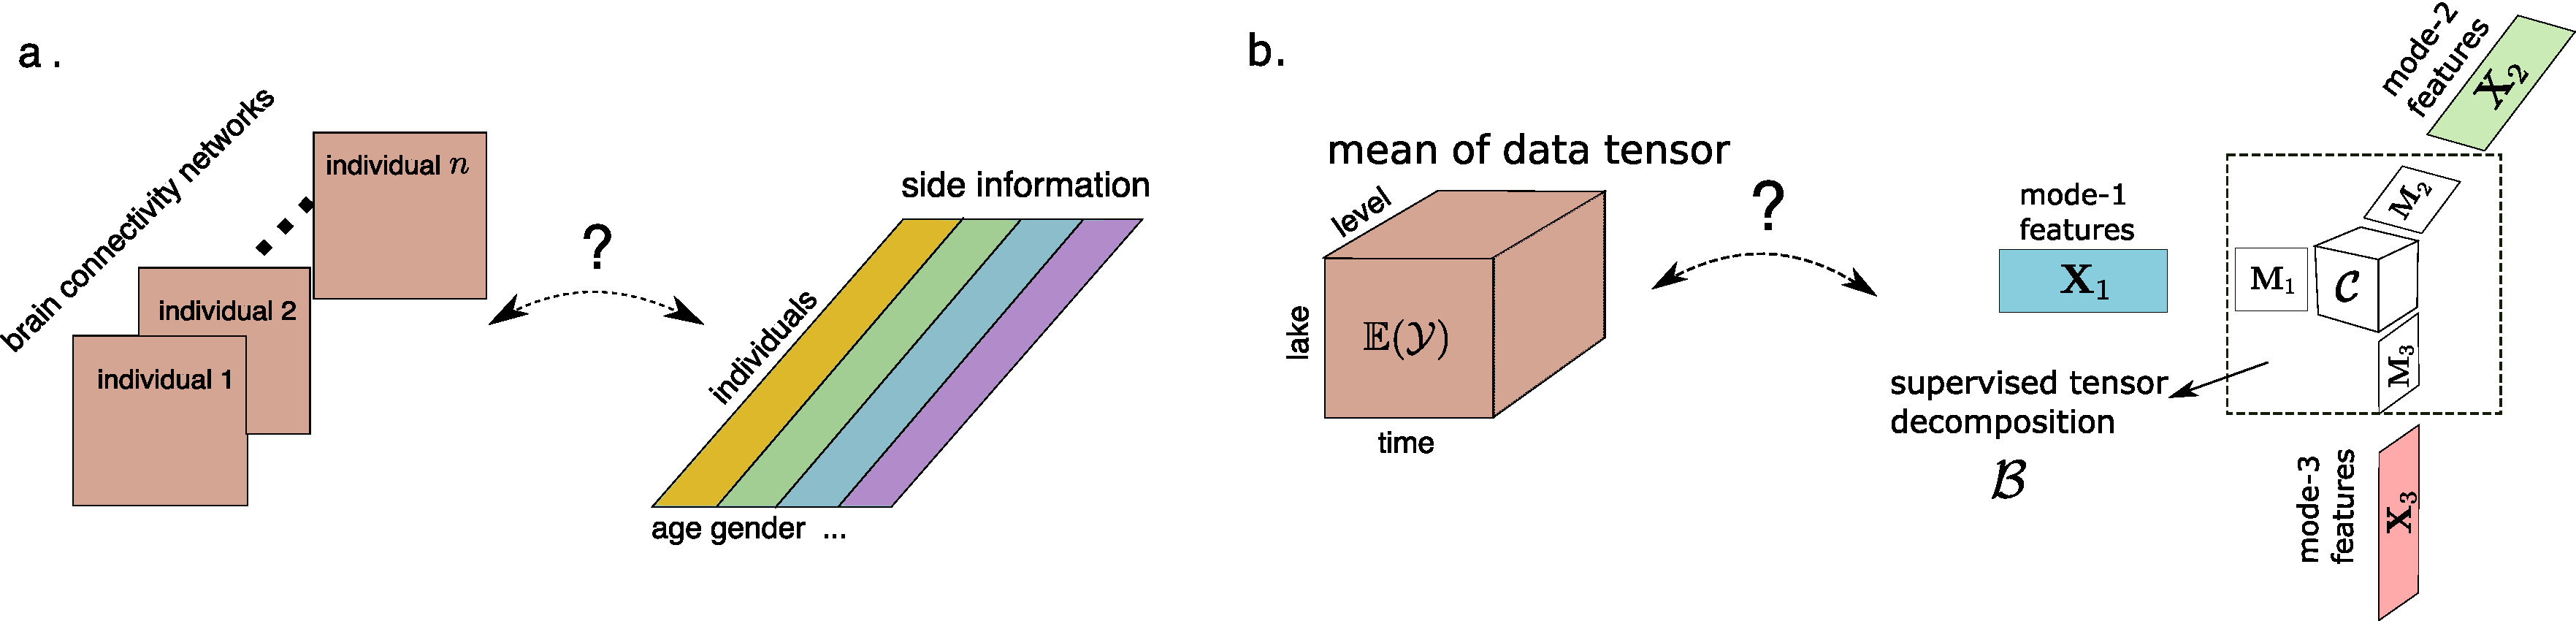
\includegraphics[width=16cm]{demo.pdf}
\end{center}
\caption{Examples of supervised tensor decomposition with interactive side information. (a) Network population model. (b) Spatio-temporal growth model.} \label{fig:intro1}
\end{figure*}

We present a general model and associated method for decomposing a data tensor whose entries are from exponential family with interactive side information. We formulate the learning task as a structured regression problem, with tensor observation serving as the response, and the multiple side information as interactive features. Figure~\ref{fig:intro1}b illustrates our model in the special case of order-3 tensors. A low-rank structure is imposed to the conditional mean of tensor observation, where unlike classical decomposition, the tensor factors $\mX_k\mM_k\in\mathbb{R}^{d_k\times r_k}$ belong to the space spanned by features $\mX_k\in\mathbb{R}^{d_k\times p_k}$ for $k=1,2,3$. The unknown matrices $\mM_k\in\mathbb{R}^{p_k\times r_k}$ (referred to as ``dimension reduction matrices'') link the conditional mean to the feature spaces, thereby allowing the identification of variations in the tensor data attributable to the side information.


Our proposal blends the modeling power of generalized linear model (GLM) and the exploratory capability of tensor dimension reduction in order to take the best out of both worlds. We leverage GLM to allow heteroscedacity due to the mean-variance relationship in the non-Gaussian data. This flexibility is important in practice. Furthermore, our low-rank model on the (transformed) conditional mean tensor effectively mitigates the curse of high dimensionality. In classical GLM, the sample size and feature dimension are well defined; however, in the tensor data analysis, we observe only one realization of an order-$K$ tensor and up to $K$ interactive feature matrices. Both the number of tensor entries and feature dimension grow exponentially in $K$. Dimension reduction is therefore crucial for prediction and interpretability. We establish the statistical convergence of our estimator, and we quantify the gain in prediction through simulations and case studies. 
 
Our work is closely related to but also clearly distinctive from several lines of previous work. The first line is a class of \textit{unsupervised} tensor decomposition such as Tucker and CP decomposition~\citep{de2000multilinear, kolda2009tensor, hong2020generalized,wang2017tensor,bi2018recom,chi2012tensors} that aims to find the best low-rank representation of a data tensor. In contrast, our model is a \textit{supervised} tensor learning, which aims to identify the association between a data tensor and multiple features. The low-rank factorization is determined jointly by the tensor data and feature matrices in our model.

The second line of work studies the tensor-on-tensor regression~\citep{raskutti2019convex, lock2018tensor,gahrooei2020multiple}. Our model shares a common ground with earlier approaches, but we provide more efficient solutions to new settings that have more practical significance. As we show in Section~\ref{sec:connection}, the supervised tensor decomposition has an interesting connection with tensor-on-tensor regression. Previous methods~\citep{lock2018tensor,lock2018supervised} mainly focus on Gaussian tensors. The Frobenius norm used in the objective function is statistical suboptimal for general exponential family tensors. Maximum likelihood estimator (MLE) is studied in~\cite{raskutti2019convex} and a convex relaxation algorithm is proposed to solve for low-rank tensor coefficients. However, in the tensor case, convex MLE suffers from both computational intractability and statistical suboptimality. We advocate a non-convex approach and provide strong evidence for its success in our setting. Most previous tensor regression focuses on prediction~\citep{lock2018tensor,raskutti2019convex}, and we go step further by finding the sufficient dimension reduction~\citep{adragni2009sufficient}, $\textup{Span}(\mM_k)$, that facilitates the identification of interaction effects in features (see Figure~\ref{fig:intro1}b). The latter approach greatly improves the \emph{interpretability} in prediction. In this regards, our method opens up new opportunities for tensor data analysis in a wider range of applications. 

The third line of work uses side information for various tensor learning tasks, such as for completion~\citep{narita2012tensor,song2019tensor,cao2016semi} and for recommendation system~\citep{ioannidis2019coupled,farias2019learning}. These methods also study tensors with side information, but they take regularization approaches to penalize predictions that are distant from side information~\citep{cao2016semi,song2019tensor}. One important difference is that their goal is prediction but not parameter estimation. The effects of features and their interactions are not estimated in these data-driven approaches. In contrast, our goal is interpretable prediction, and we estimate factor matrices $\mM_k$ using a model-based approach. Estimating $\mM_k$ allows us to identify sufficient features and the interactions thereof. We numerically compare these two approaches in Section~\ref{sec:simulation}.

The remainder of the paper is organized as follows. Section~\ref{sec:pre} introduces tensor preliminaries. Section~\ref{sec:model} presents the main model and three motivating examples for supervised tensor decomposition. We describe the quasi-likelihood estimation and alternating optimization algorithm in Section~\ref{sec:est}. In Section~\ref{sec:simulation}, we present numerical experiments and assess the performance in comparison to alternative methods. In Section~\ref{sec:data}, we apply the method to diffusion tensor imaging data from human connectome project and multi-relational social network data. We conclude in Section~\ref{sec:con} with discussions about our findings and avenues of future work. All proofs are deferred to Supplementary Materials. 

\section{Preliminaries}\label{sec:pre}
We introduce the basic tensor properties~\citep{kolda2009tensor} used in the paper. We use lower-case letters (e.g.,\ $a,b,c$) for scalars and vectors, upper-case boldface letters (e.g.,\ $\mA, \mB, \mC$) for matrices, and calligraphy letters (e.g.,\ $\tA, \tB, \tC$) for tensors of order three or greater. Let $\tY=\entry{y_{i_1,\ldots,i_K}}\in \mathbb{R}^{d_1\times \cdots\times d_K}$ denote an order-$K$ $(d_1,\ldots,d_K)$-dimensional tensor, where $K$ is the number of modes and also called the order. The multilinear multiplication of a tensor $\tY\in\mathbb{R}^{d_1\times \cdots\times d_K}$ by matrices $\mX_k=\entry{x_{i_k,j_k}^{(k)}}\in\mathbb{R}^{p_k\times d_k}$ is defined as 
\[
\tY \times_1\mX_1\times \cdots \times_K \mX_K=\entry{\sum_{i_1,\ldots,i_K}y_{i_1,\ldots,i_K}x_{j_1,i_1}^{(1)}\cdots x_{j_K,i_K}^{(K)}},
\]
which results in an order-$K$ $(p_1,\ldots,p_K)$-dimensional tensor. For ease of presentation, we use the shorthand $\tY\times\{\mX_1,\ldots,\mX_K\}$ to denote the tensor-by-matrix product. For any two tensors $\tY=\entry{y_{i_1,\ldots,i_K}}$, $\tY'=\entry{y'_{i_1,\ldots,i_K}}$ of identical order and dimensions, their inner product is defined as 
\[
\langle \tY,\ \tY'\rangle =\sum_{i_1,\ldots,i_K}y_{i_1,\ldots,i_K}y'_{i_1,\ldots,i_K}.
\]
The tensor Frobenius norm and maximum norm are defined as
\[
\FnormSize{}{\tY}=\langle \tY,\ \tY \rangle^{1/2},\quad \text{and}\quad \mnormSize{}{\tY}=\max_{i_1,\ldots,i_K}y_{i_1,\ldots,i_K}.
\]
When $a$ is a vector, we use $\vnormSize{}{a}=\langle a,a \rangle^{1/2}$ to denote the vector 2-norm. 

A higher-order tensor can be reshaped into a lower-order object. We use $\textup{vec}(\cdot)$ to denote the operation that reshapes the tensor into a vector, and $\text{Unfold}_k(\cdot)$ to denote the operation that reshapes the tensor along mode $k$ into a matrix of size $d_k$-by-$\prod_{i\neq k}d_i$. The multilinear rank of an order-$K$ tensor $\tY$ is defined as a length-$K$ vector $\mr=(r_1,\ldots,r_K)$, where $r_k$ is the rank of matrix $\textup{Unfold}_k(\tY)$, $k=1,\ldots,K$. We use $\sigma_{\min}(\cdot)$ and $\sigma_{\max}(\cdot)$ denote the smallest and largest matrix singular values. We let $\mI_d$ denote the $d \times d$ identity matrix and $[d]$ denote the $d$-set $\{1,\ldots,d\}$. We use $\mathbb{O}_{d,r}$ to denote the collection of all $d$-by-$r$ matrices with orthogonal columns; i.e., $\mathbb{O}_{d,r}=\{\mP\in\mathbb{R}^{d\times r}\colon \mP^T\mP = \mathbf{1}_r\}$. For ease of notation, we allow the basic arithmetic operators (e.g.,\ $+, -, \geq $) and univariate functions $f\colon \mathbb{R}\to \mathbb{R}$ to be applied to tensors in an element-wise manner. 
%We use $f'(\cdot)$, $f''(\cdot)$ to denote the first-order and second-order derivative of a function $f(\cdot)$. 

\section{Motivation and model}\label{sec:model}
\subsection{General framework for supervised tensor decomposition}
We begin with a general framework for supervised tensor decomposition and then discuss its implication in three concrete examples. Let $\tY=\entry{y_{i_1,\ldots,i_K}}\in\mathbb{R}^{d_1\times \cdots\times d_K}$ denote an order-$K$ data tensor. Suppose the side information is available on each of the $K$ modes. Let $\mX_k=\entry{x_{ij}}\in\mathbb{R}^{d_k\times p_k}$ denote the feature matrix on the mode $k\in[K]$, where $x_{ij}$ denotes the $j$-th feature value for the $i$-th tensor entity, for $(i,j)\in[d_k]\times[p_k]$, $p_k\leq d_k$. We propose a multilinear conditional mean model between the data tensor and feature matrices. Assume that, conditional on the features $\mX_k$, the entries of tensor $\tY$ are independent realizations from an exponential family distribution, and the conditional mean tensor admits the form
\begin{align}\label{eq:tensormodel}
&\mathbb{E}(\tY|\mX_1,\ldots,\mX_K)=f(\Theta),\quad \text{with}\quad \Theta =\tB\times\{\mX_1,\ldots, \mX_K\} ,
\end{align}
where $\Theta\in\mathbb{R}^{d_1\times \cdots\times d_K}$ is the multilinear predictor, $\tB\in\mathbb{R}^{p_1\times \cdots \times p_K}$ is the unknown parameter tensor, $f(\cdot)$ is a known link function whose form depending on the data type of $\tY$, and $\times$ denotes the tensor-by-matrix product. The choice of link function is based on the assumed distribution family of tensor entries. Common choices of link functions include identity link for Gaussian distribution, logistic link for Bernoulli distribution, and $\exp(\cdot)$ link for Poisson distribution. In general, dispersion parameters can also be included in the model. Because our main focus is the tensor decomposition under the mean model, we omit the dispersion parameter in this section for ease of presentation. 


In classical tensor decomposition, tensor factorization is performed on either data tensor $\tY$ or mean tensor $\mathbb{E}(\tY)$. In the context of supervised tensor decomposition, we propose to factorize the latent parameter tensor $\tB$,
\begin{equation}\label{eq:factor}
\tB=\tC\times\{\mM_1,\ \ldots,\ \mM_K\},
\end{equation}
where $\tC\in\mathbb{R}^{r_1\times \cdots \times r_K}$ is a full-rank core tensor, and $\mM_k\in\mathbb{R}^{p_k\times r_k}$ are factor matrices consisting of orthonormal columns, where $r_k\leq p_k$ for all $k\in[K]$. By the definition of multilinear rank, model equations~\eqref{eq:tensormodel} and~\eqref{eq:factor} imply the low-rankness $\mr=(r_1,\ldots,r_K)$ of the conditional mean tensor under the link function. We now reach our final model for supervised tensor decomposition,
\begin{align}\label{eq:decomp}
\mathbb{E}(\tY|\mX_1,\ldots,\mX_K) &= f\left(\tC\times\{\mX_1\mM_1, \ldots, \mX_K\mM_K\}\right),\notag\\
\text{with} \ &\ \mM_k^T\mM_k = \mI_{r_k},\ \mM_k\in\mathbb{R}^{p_k\times r_k}\quad \text{for all }k=1,\ldots,K,
\end{align}
where the parameters of interest are $\mM_k$ and $\tC$. Note that model~\eqref{eq:decomp} assumes a fixed, known rank $\mr=(r_1,\ldots,r_K)$; the adaptation to unknown rank will be addressed in Section~\ref{sec:tuning}. Figure~\ref{fig:intro1}b provides a schematic illustration of our model. The features $\mX_k$ affect the distribution of tensor entries in $\tY$ through the form $\mX_k\mM_k$, which are $r_k$ linear combinations of features on mode $k$. We call $\mX_k\mM_k$ the ``supervised tensor factors'' or ``sufficient features''~\citep{adragni2009sufficient}, and call $\mM_k$ the ``dimension reduction matrix.'' The core tensor $\tC$ collects the interaction effects between sufficient features across $K$ modes. Our goal is to find $\mM_k$ and the corresponding $\tC$. Note that $\mM_k$ and $\tC$ are identifiable only up to orthonormal transformations.  



\subsection{Three examples}
We give three seemingly different examples that can all be formulated as our supervised tensor decomposition model~\eqref{eq:decomp}.
\begin{example}[Spatio-temporal growth model]
The growth curve model~\citep{gabriel1998generalised,srivastava2008models} was originally proposed as an example of bilinear model for matrix data, and we adopt its higher-order extension here. Let $\tY=\entry{y_{ijk}}\in\mathbb{R}^{d \times m\times n}$ denote the pH measurements of $d$ lakes at $m$ levels of depth and for $n$ time points. Suppose the sampled lakes belong to $q$ types, with $p$ lakes in each type. Let $\{\ell_j\}_{j\in[m]}$ denote the sampled depth levels and $\{t_k\}_{k\in[n]}$ the time points. Assume that the expected pH trend in depth is a polynomial of order at most $r$ and that the expected trend in time is a polynomial of order $s$. Then, the conditional mean model for the spatio-temporal growth can be represented as
\begin{equation}\label{eq:time}
\mathbb{E}(\tY|\mX_1,\mX_2,\mX_3)=\tC\times\{\mX_1\mM_1,\ \mX_2\mM_2,\ \mX_3\mM_3\},
\end{equation}
where $\mX_1=\text{blockdiag}\{\mathbf{1}_p,\ldots,\mathbf{1}_p\}\in \{0,1\}^{d\times q}$ is the design matrix for lake types, and
\[
\mX_2=
\begin{pmatrix}
1 & \ell_1&\cdots &\ell^{r}_1\\
1 & \ell_2&\cdots &\ell^{r}_2\\
\vdots &\vdots&\ddots&\vdots\\
1&\ell_{m}&\cdots&\ell^{r}_{m}
\end{pmatrix},\quad
\mX_3=
\begin{pmatrix}
1 & t_1&\cdots &t^{s}_1\\
1 & t_2&\cdots &t^{s}_2\\
\vdots &\vdots&\ddots&\vdots\\
1&t_{n}&\cdots&t^{s}_{n}
\end{pmatrix}
\]
are the design matrices for spatial and temporal effects, respectively, $\tC\in\mathbb{R}^{r_1\times r_2\times r_3}$ is the unknown core tensor, and $\mM_k$ are unknown dimension reduction matrices on each mode. The factors $\mX_k\mM_k$ are sufficient features in the mean model~\eqref{eq:time}. The spatial-temporal model is a special case of our supervised tensor decomposition model~\eqref{eq:decomp}, with features available on each of the three modes.
\end{example}


\begin{example}[Network population model]\label{example:brain}
Network response model~\citep{rabusseau2016low} is recently developed for neuroimaging analysis. The goal is to study the relationship between brain network connectivity pattern and features of individuals. Suppose we have a sample of $n$ observations, $\{(\mY_i, \mx_i)\colon i=1,\ldots,n\}$, where for each individual $i\in[n]$, $\mY_i\in\{0,1\}^{d\times d}$ is the undirected adjacency matrix whose entries indicate presences/absences of connectivities between $d$ brain nodes, and $\mx_i\in\mathbb{R}^p$ is the individual's feature such as age, gender, cognition score, etc. The network-response model  has the conditional mean
\begin{equation}\label{eq:network}
\textup{logit}(\mathbb{E}(\mY_i|\mx_i))=\tB\times_3\mx_i, \quad \text{for }i=1,\ldots,n,
\end{equation}
where $\tB\in \mathbb{R}^{d\times d\times p}$ is a rank-$(r_1,r_1,r_2)$ coefficient tensor, and $\tB$ is assumed to be symmetric in the first two modes.  

The model~\eqref{eq:network} is a special case of our supervised tensor decomposition, with feature matrix on the last mode of the tensor. Specifically, we stack the network observations $\{\mY_i\}$ together and obtain an order-3 response tensor $\tY\in\{0,1\}^{d\times d\times n}$. Define a feature matrix $\mX=[\mx_1,\ldots,\mx_n]^T\in\mathbb{R}^{n\times p}$. Then, the model~\eqref{eq:network} has the equivalent representation of supervised tensor decomposition,
\[
\textup{logit}(\mathbb{E}(\tY|\mX))=\tC\times\{\mM,\ \mM,\ \mX\mM'\},
\]
where $\tC\in\mathbb{R}^{r_1\times r_1\times r_2}$ is the core tensor, $\mM\in\mathbb{R}^{d\times r}$ is the dimension reduction matrix on the first two modes, and $\mM'\in\mathbb{R}^{p\times r_2}$ is for the last mode.  \end{example}
 
 \begin{example}[Dyadic data with node attributes] Dyadic dataset consists of measurements on pairs of objects. Common examples include graphs and networks. Let $\tG=(V,E)$ denote a graph, where $V=[d]$ is the node set of the graph, and $E\subset V\times V$ is the edge set. Suppose that we also observe feature vector $\mx_i\in\mathbb{R}^p$ associated to each node $i\in V$. A probabilistic model on the graph $\tG=(V,E)$ can be described by the following matrix regression. The edge connects the two vertices $i$ and $j$ independently of other pairs, and the probability of connection is modeled as
\begin{equation}\label{eq:edge}
 \textup{logit}\left(\mathbb{P}\left((i,j)\in E\right)\right)=\mx^T_i\mB\mx_j=\langle \mB,\ \mx^T_i\mx_j\rangle,
 \end{equation}
 where $\mB\in\mathbb{R}^{p\times p}$ is a symmetric rank-$r$ matrix. The low-rankness in $\mB$ has demonstrated its success in modeling transitivity, balance, and communities in  networks~\citep{hoff2005bilinear}. We show that our supervised tensor decompostion~\eqref{eq:decomp} also incorporates the graph model as a special case. Let $\tY=\entry{y_{ij}}$ be a binary matrix where $y_{ij}=\mathds{1}_{(i,j)\in E}$. Define $\mX=[\mx_1,\ldots,\mx_n]^T\in\mathbb{R}^{n\times p}$. Then, the graph model~\eqref{eq:edge} can be expressed as
 \[
 \textup{logit}(\mathbb{E}(\mY|\mX))=\mC\times\{\mX\mM,\ \mX\mM\}, 
  \]
  where $\mC\in\mathbb{R}^{r\times r}, \mM\in\mathbb{R}^{p\times r}$ are from the singular value decomposition of $\mB=\mM\mC\mM^T$. 
  \end{example}


%In the above three examples and many other studies, researchers are interested in uncovering the variation in the data tensor that can be explained by features. The coefficient tensor $\tB$ in model~\eqref{eq:tensormodel} serves this goal by collecting the feature effects. To encourage the sharing among effects, decomposition~\eqref{eq:factor} assumes that the feature effects $\tB$ lie in a low-dimensional parameter space. The low-rank assumption is plausible in many scientific applications. In the Example~\ref{example:brain} of brain imaging analysis, for instance, it is often believed that the brain nodes can be partitioned into several regions, and the person's attributes affect the connectivity in a similar way within a region. 


In the above three examples and many other studies, researchers are interested in uncovering the variation in the data tensor that can be explained by features. Our supervised tensor decomposition~\eqref{eq:decomp} allows arbitrary numbers of feature matrices. When certain mode $k$ has no side information, we set $\mX_k=\mI_{d_k}$ in the model~\eqref{eq:decomp}. In particular, our model~\eqref{eq:decomp} reduces to classical unsupervised tensor decomposition~\citep{de2000multilinear,hong2020generalized} when no side information is available; i.e., $\mX_k=\mI_{d_k}$ for all $k\in[K]$.


\subsection{Connection to sufficient dimension reduction and tensor-on-tensor regression}\label{sec:connection}
One important implication of our method is that we allow high-dimensionality in both tensor dimension $d_k$ and feature dimension $p_k$. Recall that the model rank $r_k$ is typically smaller than $d_k$ and $p_k$. In such a case, the matrices $\mM_k$ serve the role of simultaneous dimension reduction of the data tensor and features. The role of the sufficient features $\mX_k\mM_k$ can be seen in the following two conditional independence assumptions in model~\eqref{eq:decomp},
\begin{align}
\tY \ci \{\mX_k\}&\ \big|\ \{\mX_k\mM_k\} \ \ \text{(independence between the tensor and features)},\\
y_{i_1,\ldots,i_K} \ci y_{i'_1,\ldots,i'_K} & \ \big|\ \{\mX_k\mM_k\}  \ \ \text{(independence within the tensor)},
\end{align}
where the second line holds for all $(i_1,\ldots,i_K)\neq(i'_1,\ldots,i'_K) \in[d_1]\times\cdots\times[d_K]$, and $\ci$ denotes the independence. The first property highlights the ``decorrelation'' role of $\mM_k$, in the same spirit as the sufficient dimension reduction~\citep{adragni2009sufficient} in supervised learning, whereas the second property highlights the tensor dimension reduction in the usual unsupervised sense (consider, for example, $\mX_k=\mathbf{I}_{d_k}$ for all $k\in[K]$).

Our model also has a close connection with tensor-on-tensor regression~\citep{raskutti2019convex, lock2018tensor,gahrooei2020multiple,hao2020sparse}. Specifically, model~\eqref{eq:decomp} can be viewed as a multivariate regression model, where the response is the vectorized tensor and the covariates are interactions between sufficient features across modes. We take an order-3 tensor under the Gaussian model for illustration. Let $\mX,\mZ,\mW$ denote the feature matrix on mode $k=1, 2, 3$, respectively. Suppose that each mode has two-dimensional sufficient features, denoted $\mM_1\mX=[\mx_1,\mx_2]$, $\mM_2\mZ=[\mz_1,\mz_2]$, $\mM_3\mW=[\mw_1,\mw_2]$. Here $\mx_1,\mx_2,\ldots,\mw_1, \mw_2$ are column vectors. Then the model~\eqref{eq:decomp} is a regression model with across-mode interactions,
\begin{equation}\label{eq:interaction}
\mathbb{E}(y_{ijk}|\mX,\mZ,\mW)=c_{111}\mx_{1i}\mz_{1j}\mw_{1k}+c_{121}\mx_{i1}\mz_{j2}\mw_{k1}+\cdots+c_{221}\mx_{2i}\mz_{2j}\mw_{1k}+c_{222}\mx_{2i}\mz_{2j}\mw_{2k},
\end{equation}
where $\entry{c_{ijk}} \in \mathbb{R}^{2\times 2\times 3}$ are unknown interaction effects, $\mx_{1i}$ denotes the $i$-th entry in the feature vector $\mx_1$, and similar notations apply to other features. Note that lower-order interactions are naturally incorporated in~\eqref{eq:interaction} if we include an intercept column in the sufficient feature matrices. Model~\eqref{eq:interaction} shows the benefit of our supervised tensor decomposition for identifying across-mode interactions. 

\section{Estimation}\label{sec:est}

\subsection{Rank-constrained M-estimator}
We develop a likelihood-based procedure to estimate $\tC$ and $\mM_k$ in~\eqref{eq:decomp}. We adopt the exponential family as a flexible framework for different data types. In a classical generalized linear model with a scalar response $y$ and feature $\mx$, the density is expressed as
\[
p(y|\mx, \boldsymbol{\beta})=c(y,\phi)\exp\left(\frac{y\theta- b(\theta)}{\phi}\right)\ \text{with}\ \theta=\boldsymbol{\beta}^T\mx,
\]
where $b(\cdot)$ is a known function, $\theta$ is the linear predictor, $\phi>0$ is the dispersion parameter, and $c(\cdot)$ is a known normalizing function. The choice of link functions depends on the data types and on the observation domain of $y$, denoted $\mathbb{Y}$. For example, the observation domain is $\mathbb{Y}=\mathbb{R}$ for continuous data, $\mathbb{Y}=\mathbb{N}$ for count data, and  $\mathbb{Y}=\{0,1\}$ for binary data. The canonical link function $f$ is chosen to be $f(\cdot)=b'(\cdot)$, the first-order derivative of $b(\cdot)$. Table~1 summarizes the canonical link functions for common types of distributions. 

\begin{table}[htb]
\centering
\begin{tabular}{c|ccc}
Data type &Gaussian & Poisson& Bernoulli\\
\hline
Domain $\mathbb{Y}$& $\mathbb{R}$&$\mathbb{N}$&$\{0,1\}$\\
 $b(\theta)$&$\theta^2/2$& $\exp(\theta)$&$\log (1+\exp(\theta))$\\
 link $f(\theta)$&$\theta$&$\exp(\theta)$&$(1+\exp(-\theta))^{-1}$
\end{tabular}
\caption{Canonical links for common distributions.}\label{table:link}
\end{table}


In our context, we model the tensor entries $y_{i_1,\ldots,i_K}$, conditional on $\theta_{i_1,\ldots,i_K}$, as independent draws from an exponential family. Ignoring constants that do not depend on $\Theta$, the quasi log-likelihood of~\eqref{eq:decomp} is equal to Bregman distance between $\tY$ and $b'(\Theta)$:
\begin{align}\label{eq:loglikelihood}
\tL_{\tY}(\tC,\mM_1,\ldots,\mM_K)&=\langle \tY, \Theta \rangle - \sum_{i_1,\ldots,i_K} b(\theta_{i_1,\ldots,i_K}),\\
 \text{where}\quad \Theta&=\tC\times\{\mM_1\mX_1,\ldots,\mM_K\mX_K\}.
\end{align}
We propose a constrained maximum quasi-likelihood estimator (M-estimator),
\begin{align} \label{eq:MLE} 
(\hat \tC, \hat \mM_1,\ldots,\hat \mM_k) &=\argmax_{(\tC,\mM_1,\ldots,\mM_K)\in \tP} \ \tL_{\tY}(\tC,\mM_1,\ldots,\mM_K),
\end{align}
where the parameter space $\tP$ is
\[
\tP=\left\{(\tC, \mM_1,\ldots,\mM_K) \ \Big| \ \mM_k^T\mM_k=\mathbf{I}_{r_k}\ \text{for all }k\in[K],\  \mnormSize{}{\Theta(\tC,\mM_1,\ldots,\mM_K)}\leq \alpha \right\}.
\]
The maximum norm constraint on the linear predictor $\Theta$ is a technical condition to avoid the divergence in the non-Gaussian variance.


\subsection{Alternating optimization} \label{subsec:alg}
We propose an alternating optimization algorithm to solve~\eqref{eq:MLE}. 
The decision variables in the objective function~\eqref{eq:MLE} consist of $K+1$ blocks of variables, one for the core tensor $\tC$ and $K$ for the factor matrices $\mM_k$. We notice that, if any $K$ out of the $K+1$ blocks of variables are known, then the optimization reduces to a simple GLM with respect to the last block of variables. This observation leads to an iterative updating scheme for one block at a time while keeping others fixed. After each iteration, we rescale the core tensor $\tC^{(t+1)}$ subject to the maximum norm constraint. The full algorithm is described in Algorithm~\ref{alg:B}. 



\begin{algorithm}[!h]
\caption{Supervised Tensor Decomposition with Interactive Side Information}\label{alg:B}
\begin{algorithmic}[1]
\INPUT Response tensor $\tY\in \mathbb{R}^{d_1\times \cdots \times d_K}$, feature matrices $\mX_k\in\mathbb{R}^{d_k\times p_k}$ for $k=1,\ldots,K$, target Tucker rank $\mr=(r_1,\ldots,r_K)$, link function $f$, maximum norm bound $\alpha$
\OUTPUT Estimated core tensor $\hat \tC\in\mathbb{R}^{r_1\times \cdots \times r_K}$ and factor matrices $\hat \mM_k\in\mathbb{R}^{p_k\times r_k}$. 
\State Random initialization of the core tensor $\tC$ and factor matrices $\mM_k$. 
\While{Do until convergence}
\For { $k=1$ to $K$}
\State Obtain the factor matrix $\tilde \mM_k\in\mathbb{R}^{p_k\times r_k}$ by a GLM with link function $f$.
\State Perform QR factorization $\tilde \mM_k=\mQ\mR$, where $\mQ\in\mathbb{R}^{p_k\times r_k}$ consists of orthonormal columns.
\State Update $\mM_k\leftarrow \mQ$ and core tensor $\tC\leftarrow \tC\times_k \mR$.
\EndFor
\State Update the core tensor $\tC$ by solving a GLM with $\textup{vec}(\tY)$ as response, $\otimes_{k=1}^K[ \mX_k\mM_k]$ as features, and $f$ as link function. Here $\otimes$ denotes the Kronecker product of matrices. 
\State Rescale the core tensor $\tC$ subject to the maximum norm constraint. 
\EndWhile
\end{algorithmic}
\end{algorithm}

The optimization~\eqref{eq:MLE} is a non-convex problem due to the non-convexity in the feasible set $\tP$. Under mild conditions, our algorithm enjoys global convergence; i.e.\ any sequence of iterates generated by the alternating algorithm converges to a stationary point of $\tL_\tY(\cdot)$ module orthogonal transformation. To establish the convergence properties of Algorithm~\ref{alg:B}, we first introduce the equivalent relationship induced by orthogonal transformation. 

\begin{defn}[Equivalence class]Let $\tA = (\tC, \mM_1,\ldots,\mM_K) \in \mathbb{R}^{d_{\text{total}}}$ denote the collection of decision variables in the alternating optimization, where $d_{\text{total}} = \prod_k r_k + \sum_k r_kd_k$. 
Two parameters $\tA'=(\tC', \mM'_1,\ldots,\mM'_k)$ and $\tA=(\tC, \mM_1,\ldots,\mM_k)$ are called equivalent, denoted $\tA\sim \tA'$, if and only if there exist orthogonal matrices $\mP_k \in \mathbb{O}_{d_k,r_k}$ such that
\begin{align}\label{eq:equivalance}
	\mM'_k \mP^T_k = \mM_k \quad \text{for all }k \in [K], \quad \text{and}\quad \tC' \times_1 \mP_1 \times_2  \dots \times_K \mP_K = \tC.
\end{align}
Equivalently, two parameters $\tA,\ \tA'$ are equivalent if the corresponding Tucker tensors~\eqref{eq:factor} are the same, $\tB(\tA)=\tB'(\tA')$. 
\end{defn}

\begin{prop}[Global convergence]\label{prop:alg}
Assume the set $\{\tA\ |\ \tL_\tY(\tA) \geq \tL_\tY(\tA^{(0)}) \}$ is compact and the stationary points of $\tL_\tY(\tA)$ are isolated module the equivalence defined in~\eqref{eq:equivalance}. Furthermore, assume that $\alpha = \infty$; i.e., we impose no entrywise bound constrains on the parameter space. Then any sequence $\tA^{(t)}$ generated by Algorithm~\ref{alg:B} converges to a stationary point of $\tL_\tY(\tA)$ module equivalence class.
\end{prop}


In theory, global optimality of non-convex optimization is often challenging to obtain. Fortunately, we will show in Section~\ref{subsec:statprob} that the desired statistical performance holds for all local optimizers satisfying $\tL_{\tY}(\hat \tC, \hat \mM_1,\ldots,\hat \mM_K)\geq \tL_{\tY} (\tC_{\textup{true}},\mM_{1,\textup{true}},\ldots,\mM_{K,\textup{true}})$, where the subscript ``true'' denotes the true parameter in model~\eqref{eq:decomp}. This result indicates the global optimality is not necessarily a serious concern in our context, as long as the convergent objective is large enough. In the experiments we considered, we find that Algorithm~\ref{alg:B} typically gives satisfactory convergent points upon random initialization. Figure~\ref{fig:loglike} shows the trajectories of objective function for order-3 tensors based on model~\eqref{eq:decomp}, where $d_k = d \in\{25,30\}$, $p_k = 0.4d$, $r_k = r\in\{3,6\}$ for $ k = 1,2,3$. We consider input tensors with Gaussian, Bernoulli, and Poisson entries. Under all combinations of the dimension $d$, rank $r$, and type of the entries, Algorithm~\ref{alg:B} converges quickly in a few iterations, and the objective values at convergent points are close to or larger than the value at true parameters.  

\begin{figure}[t]
\centering
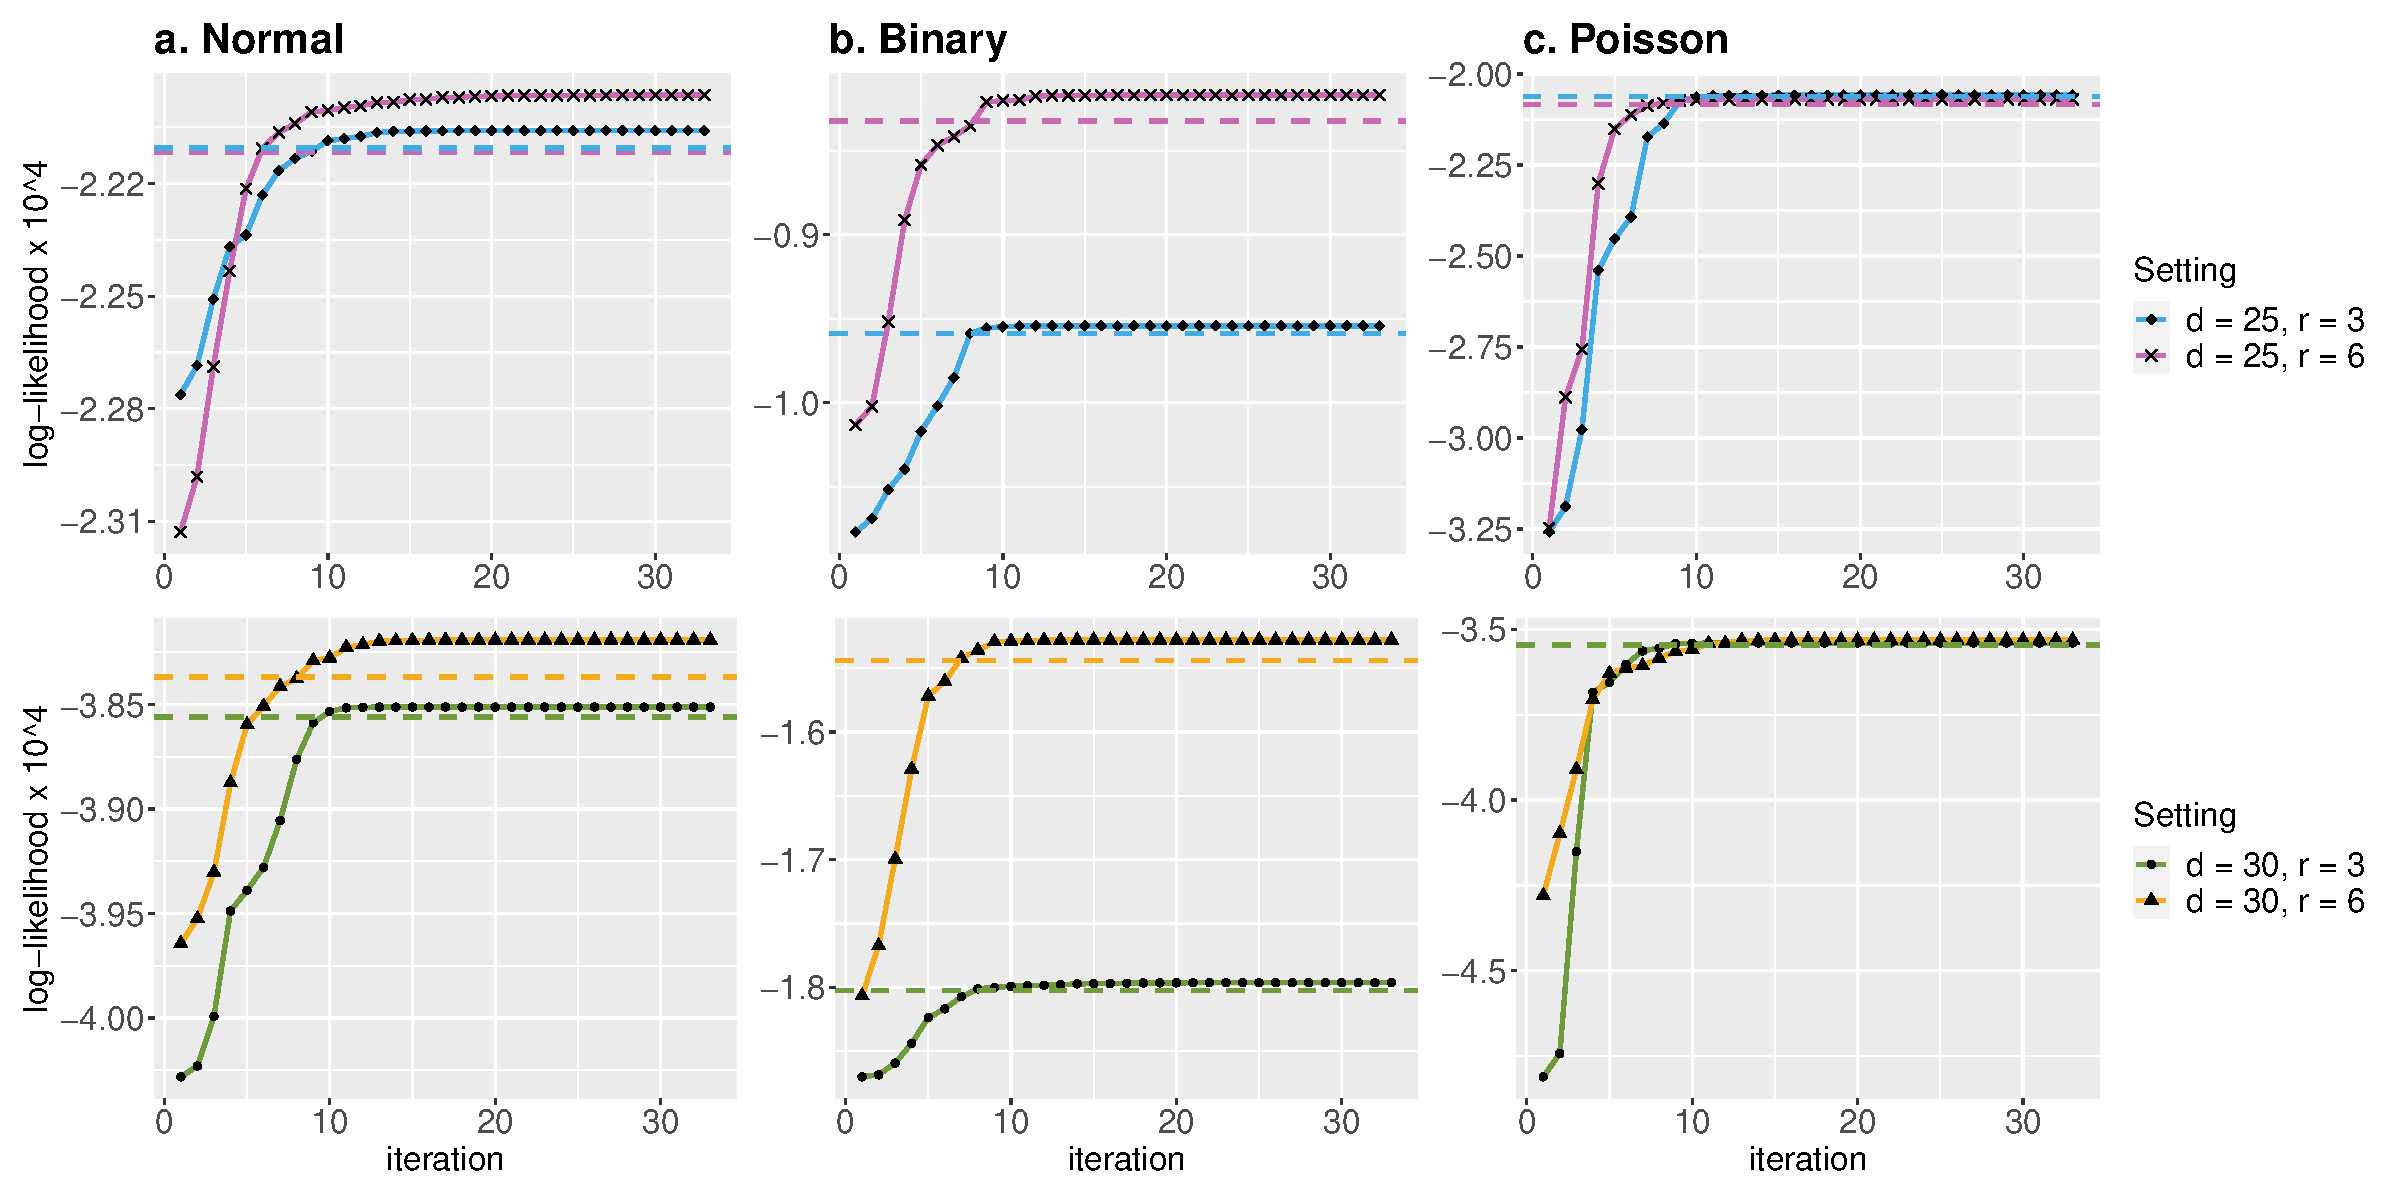
\includegraphics[width=16cm]{loglike.pdf}
\caption{Trajectory of the objective function with various dimension $d$ and rank $r$ under (a) Gaussian (b) Bernoulli (c) Poisson models. The dashed line represents the objective value at true parameters. }\label{fig:loglike}
\end{figure}



\subsection{Rank selection and computational complexity}\label{sec:tuning}
Algorithm~\ref{alg:B} assumes the rank $\mr$ is given. In practice, the rank is often unknown and must be determined from the data. We propose to use Bayesian information criterion (BIC) and choose the rank that minimizes BIC, where
\begin{equation}\label{eq:BIC}
%\hat \mr&=\argmin_{\mr=(r_1,\ldots,r_K)} \textup{BIC}(\mr)\notag\\
\textup{BIC}(\mr)=-2\tL_{\tY}(\hat \tC, \hat \mM_1,\ldots,\hat \mM_K)+p_e(\mr)\log (\prod\nolimits_k d_k).
\end{equation}
Here, $p_e(\mr)\stackrel{\textup{def}}{=}\sum_k (p_k-r_k-1)r_k+\prod_k r_k$ is the effective number of parameters in the model. We choose $\hat \mr$ that minimizes $\textup{BIC}(\mr)$ via grid search. Our choice of BIC aims to balance between the goodness-of-fit for the data and the degree of freedom in the population model. We evaluate the empirical performance of BIC in Section~\ref{sec:simulation}.  

The computational complexity of our Algorithm~\ref{alg:B} is $O\left(d \sum_k p^3_k\right)$ for each loop of iterations, where $d=\prod_k d_k$ is the total size of the data tensor. More precisely, the update of core tensor costs $O(r^3d)$, where $r=\prod_k r_k$ is the total size of the core tensor. The update of each factor matrix $\mM_k$ involves a GLM with a $d$-length response, and $d$-by-$(r_kp_k)$ feature matrix. Solving such a GLM requires $O(dr^3_kp^3_k)$, and therefore the cost for updating $K$ factors in total is $O( d\sum_k r^3_k p_k^3)$. This complexity in tensor dimension matches with the classical tensor decomposition~\citep{kolda2009tensor}. 



\subsection{Statistical properties}\label{subsec:statprob}
In this section, we provide the accuracy guarantee for the proposed M-estimator~\eqref{eq:MLE}. Note that the factor matrices $\mM_k$ are identifiable only up to orthogonal transformation. Therefore, we use angle distance to assess the accuracy in estimating the column space, $\textup{Span}(\mM_k)$. For any two column-orthonormal matrices $\mA,\mB\in\mathbb{O}(d,r)$ of same dimension, the angle distance is defined as
\[
\sin \Theta(\mA,\mB)=\snormSize{}{\mA^T \mB^{\perp}}=\max\left\{ \frac{\langle \mx, \my\rangle}{\vnormSize{}{\mx}\vnormSize{}{\my}}\colon \ \mx\in \textup{Span}(\mA),\ \my\in \textup{Span}(\mB^{\perp})\right\}.
\]

In modern applications, the tensor data and features are often large-scale. We are particularly interested in the high-dimensional regime in which both $d_k$ and $p_k$ diverge; i.e.\ $d_k\to \infty$ and $p_k\to\infty$, while $p_k/d_k \to \gamma_k \in[0,1)$. As the size of problem grows, and so does the number of unknown parameters. The classical MLE theory does not directly apply. We leverage the recent development in random tensor theory and high-dimensional statistics to establish the error bounds of the estimation. 

 
\begin{assumption}\label{ass}We make the following assumptions:
\begin{enumerate}[noitemsep,topsep=0pt]
\item [A1.] There exist two positive constants $c_1, c_2>0$ such that $c_1\leq \sigma_{\min}(\mX_k)\leq  \sigma_{\max}(\mX_k)\leq c_2$ for all $k\in[K]$. 
%Here $\sigma_{min}(\cdot)$ and $\sigma_{max}(\cdot)$ denote the smallest and largest matrix singular values.
\item [A1'.] The feature matrices $\mX_k$ are Gaussian designs with i.i.d.\ $N(0,1)$ entries.
\item [A2.] There exist two positive constants $L, U>0$, such that $L\phi \leq \textup{Var}(y_{i_1,\ldots,i_K}|\theta_{i_1,\ldots,i_K})\leq U\phi $, or equivalently, $L\leq b''(\theta_{i_1,\ldots,i_K}) \leq U$, for all $|\theta_{i_1,\ldots,i_K}|\leq \alpha$. Here $\alpha$ is the upper bound of the linear predictor in~\eqref{eq:MLE}, and $b''(\cdot)$ denotes the second-order derivative. 

\end{enumerate}
\end{assumption}
The assumptions are fairly mild. Assumptions A1 and A1' consider two separate scenarios about feature matrices. Assumption A1 is applicable when feature matrix is asymptotically non-singular and has bounded spectral norm, whereas Assumption A1' imposes the commonly-used Gaussian design~\citep{raskutti2019convex}. Assumption A2 ensures the log-likelihood $\tL_\tY(\Theta)$ is strictly concave in the linear predictor $\Theta$. 
%The two equivalent statements in Assumption A2 are based on the fact that $\textup{Var}(y_{i_1,\ldots,i_K}|\tX,\tB)=\phi b''(\theta_{i_1,\ldots,i_K})$ when $y_{i_1,\ldots,i_K}$ belongs to an exponential family~\citep{mccullagh1989generalized}. 

 
\begin{thm}[Statistical convergence]\label{thm:main}
Consider a data tensor generated from model~\eqref{eq:decomp}, where the entries are conditionally independent realizations from an exponential family. Let $(\hat \tC, \hat \mM_1,\ldots,\hat \mM_K)$ be the M-estimator in~\eqref{eq:MLE} and $\hat \tB=\hat \tC\times \hat \mM_1\times\cdots \times \hat \mM_K$. Define $r_\textup{total}=\prod_k r_k$ and $r_{\max}=\max_k r_k$. Under Assumptions A1 and A2 with scaled feature matrices $\check \mX_k= \sqrt{d_k}\mX_k$, or under Assumptions A1' and A2 with original feature matrices, there exist two positive constants $C_1=C_1(\alpha,K), C_2=C_2(\alpha, K)>0$ independent of dimensions $\{d_k\}$ and $\{p_k\}$, such that, with probability at least $1-\exp(-C_1\sum_k p_k)$, 
\begin{equation}\label{eq:bound}
    \FnormSize{}{\trueB- \hat \tB}^2\leq \frac{ C_{2} r_{\textup{total}}}{r_{\max}}\frac{\sum_k p_k}{\prod_k d_k}.
\end{equation}
Furthermore, if the unfolded core tensor has non-degenerate singular values at mode $k\in[K]$, i.e., $\sigma_{\min}(\textup{Unfold}_k(\tC_\textup{true})) \geq c>0$ for some constant $c$, then
\begin{equation}\label{eq:sinebound}
\textup{sin}^2 \Theta(\trueM,\ \hat \mM_k) \leq  \frac{ C_{2}r_{\textup{total}}}{ r_{\max}\sigma^2_{\min}(\textup{Unfold}_k(\tC_\textup{true}))}\frac{\sum_k p_k}{\prod_k d_k}.
\end{equation}
\end{thm}

Theorem~\ref{thm:main} establishes the statistical convergence for the estimator~\eqref{eq:MLE}. In fact, our proof shows that the desired convergence rate holds not only for the M-estimator, but also for any local optimizers satisfying $\tL_\tY(\hat \tC, \hat \mM_1,\ldots,\hat \mM_K) \geq \tL_\tY(\tC_{\textup{true}},  \mM_{1,\textup{true}},\ldots,\mM_{K,\textup{true}})$. Consider a special case when tensor dimensions are equal on each of the modes, i.e., $d_k=d$ for all $k\in[K]$, and feature dimension grows with tensor dimension, $p_k=\gamma d$, $\gamma\in [0,1)$, for $k\in[K]$. The result in~\eqref{eq:bound} implies that the estimation has a convergence rate $\tO(d^{-(K-1)})$. Therefore, our estimation is consistent in high dimensional regimes, and the convergence becomes especially favorable as the order of tensor data increases. 

As immediate applications, we obtain the convergence rate for the three examples mentioned in Section~\ref{sec:model}.

\begin{customexample}{1}[Spatio-temporal growth model] The estimated type-by-time-by-space coefficient tensor converges at the rate $\tO\left(\frac{p+r+s}{dmn}\right)$ where $p\leq d$, $r\leq m$ and $s\leq n$. The estimation achieves consistency as long as the dimension grows along either of the three modes.
\end{customexample}

\begin{customexample}{2} [Network population model] The estimated node-by-node-by-feature tensor converges at the rate $\tO\left(\frac{2d+p}{d^2n}\right)$ where $p\leq n$. The estimation achieves consistency as the number of individuals or the number of nodes grows. 
\end{customexample}

\begin{customexample}{3} [Dyadic data with node attributes] The estimated feature-by-feature matrix converges at the rate $\tO\left(\frac{p}{d^2}\right)$ where $p\leq d$. Again, our estimation achieves consistency as the number of nodes grows. 
\end{customexample}

We conclude this section by providing the accuracy, measured in KL divergence, for the response distribution.   

\begin{cor}[Prediction error]\label{thm:KL}
Assume the same set-up as in Theorem~\ref{thm:main}. Let $\mathbb{P}_{\tY_{\textup{true}}}$ and $\mathbb{P}_{\hat \tY}$ denote the distributions of $\tY$ given the true parameter $\trueB$ and estimated parameter $\hat \tB$, respectively. Then, we have, with probability at least $1-\exp(C_1\sum_k p_k)$,
\[
\textup{KL}(\mathbb{P}_{\tY_{\textup{true}}},\ \mathbb{P}_{\hat \tY})\leq \frac{C_3r_{\textup{total}}}{r_{\max}}\sum_k p_k,
\]
where $C_3=C_3(\alpha, K)>0$ is a constant independent of dimensions $\{d_k\}$ and $\{p_k\}$.
\end{cor}

\section{Numerical experiments}\label{sec:simulation}
We evaluate the empirical performance of our supervised tensor decomposition (STD) through simulations. We consider order-3 tensors with a range of distribution types. Unless otherwise specified, the conditional mean tensor is generated form model~\eqref{eq:decomp}, where the core tensor entries are i.i.d.\ drawn from Uniform[-1,1], the factor matrix $\mM_k$ is uniformly sampled with respect to Haar measure from matrices with orthonormal columns. The feature matrix $\mX_k$ is either an identity matrix (i.e.,\ no feature  available) or Gaussian random matrix with i.i.d.\ entries from $N(0,1)$. The linear predictor $\Theta=\tC\times\{\mM_1\mX_1,\mM_2\mX_3,\mM_3\mX_3\}$ is scaled such that $\mnormSize{}{\Theta}=1$. Conditional on the linear predictor $\Theta=\entry{\theta_{ijk}}$, the entries in the tensor $\tY=\entry{y_{ijk}}$ are drawn independently according to three probabilistic models:

\begin{enumerate}[noitemsep,topsep=0pt]
\item[(a)] Gaussian model: continuous tensor entries $y_{ijk}\sim N\left(\alpha \theta_{ijk}, 1\right)$.
\item[(b)] Poisson model: count tensor entries $y_{ijk}\sim\textup{Poisson}\left( e^{\alpha \theta_{ijk}}\right)$.
\item[(c)] Bernoulli model: binary tensor entries $y_{ijk}\sim \textup{Bernoulli}\left( \frac{e^{\alpha \theta_{ijk}}}{1+e^{\alpha \theta_{ijk}}}\right)$.
\end{enumerate}
Here $\alpha>0$ is a scalar controlling the magnitude of the effect size. In each simulation study, we report the mean squared error (MSE), $\FnormSize{}{\tB_{\textup{true}}-\hat \tB}^2$, averaged across $30$ replications. 

\subsection{Finite-sample performance}
The first experiment assesses the selection accuracy of our BIC criterion~\eqref{eq:BIC}. We consider the balanced situation where $d_k=d$, $p_k=0.4d_k$ for $k=1,2,3$. We set $\alpha=4$ and consider various combinations of dimension $d$ and rank $\mr=(r_1,r_2,r_3)$. For each combination, we minimize BIC using a grid search over three modes. The hyper-parameter $\alpha$ is set to infinity in the fitting, which essentially imposes no constraint on the tensor magnitude. Table~\ref{tab:rank} reports the selected rank averaged over $n_{\textup{sim}}=30$ replicates. We found that in the high-rank setting with $d=20$, the selected rank slightly underestimates the true rank, and the accuracy immediately improves when either the dimension increases to $d = 40$ or the rank reduces to $\mr = (3,3,3)$. This agrees with our expectation, because in the tensor decomposition, the sample size is related to the number of tensor entries. A larger $d$ implies a larger sample size, so the BIC selection becomes more accurate. 

\begin{table}[tb]
\resizebox{\textwidth}{!}{%
\centering
\begin{tabular}{c|cc|cc}
True Rank $\mr$ &\multicolumn{2}{c|}{Dimension (Gaussian tensors)}&\multicolumn{2}{c|}{Dimension (Poisson tensors)}\\
%True rank $\mr$& $d=20$  (Gaussian) &$d=40$ (Gaussian) &$d=20$ (Poisson) &$d=40$ (Poisson)\\
\hline
$(3,\ 3,\ 3)$&$({\bf 3.0},\ {\bf 3.0},\ {\bf 3.0})$&$({\bf 3.0},\ {\bf 3.0},\ {\bf 3.0})$& $({\bf 3.0},\ {\bf 3.0},\ {\bf 3.0})$ & $({\bf 3.0},\ {\bf 3.0},\ {\bf 3.0})$\\
$(4,\ 4,\ 6)$&$(3.0,\ 3.0,\ {\bf 4.6})$&$({\bf 4.0},\ {\bf 4.0},\ {\bf 5.3})$&$(3.0,\ 3.0,\ {\bf 5.3})$&$({\bf 4.0},\ {\bf 4.0},\ {\bf 5.6})$\\
$(6,\ 8,\ 8)$&$(5.0,\ 5.0,\ 5.0)$&$({\bf 6.0},\ {\bf 8.0},\ {\bf 8.0})$&$(5.0,\ 5.0,\ 6.7)$&$({\bf 6.0},\ {\bf 8.0},\ {\bf 8.0})$\\
\end{tabular}
}
\caption{Rank selection via BIC. The estimated ranks are averaged across 30 simulation. Bold number indicates the ground truth is within two standard deviations of the estimate.}\label{tab:rank}
\end{table}

\begin{figure}[!h]
\centering
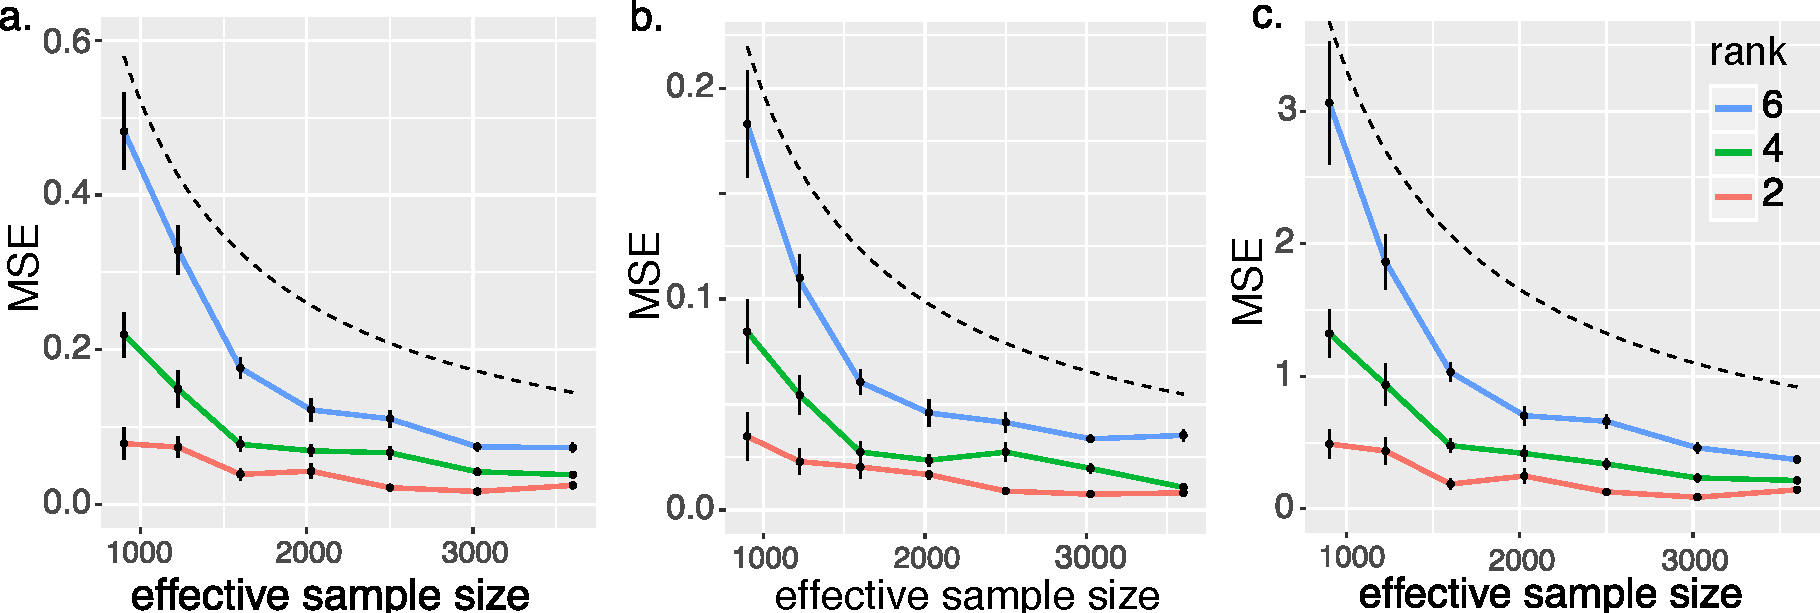
\includegraphics[width=14cm]{dimension.pdf}
\caption{Estimation error against effective sample size. The three panels plot the MSE when the response tensors are generated from (a) Gaussian (b) Poisson and (c) Bernoulli models. The dashed curves correspond to $\tO({1/d^2})$.}\label{fig:dim}
\end{figure}

The second experiment evaluates the accuracy when features are available on all modes. We set $\alpha=10, d_k=d, p_k=0.4d_k, r_k=r\in\{2,4,6\}$ and increase $d$ from 30 to 60. Our theoretical analysis suggests that $\hat \tB$ has a convergence rate $\tO(d^{-2})$ in this setting. Figure~\ref{fig:dim} plots the estimation error versus the ``effective sample size'', $d^2$, under three different distribution models. We find that the empirical MSE decreases roughly at the rate of $1/d^2$, which is consistent with our theoretical results. We also observe that, tensors with higher rank tend to yield higher estimation errors, as reflected by the upward shift of the curves as $r$ increases. Indeed, a larger $r$ implies a higher model complexity and thus greater difficulty in the estimation. 



\subsection{Comparison with GLMs under stochastic block models}
The third experiment investigates the performance of our model under correlated feature effects. We mimic the scenario of brain imaging analysis. A sample of $d_3=50$ networks are simulated, one for each individual. Each network measures the connections between $d_1=d_2=20$ brain nodes. We simulate $p=5$ features for the each of the 50 individuals. These features may represent, for example, age, gender, cognitive score, etc. Recent study has suggested that brain connectivity networks often exhibit community structure represented as a collection of subnetworks, and each subnetwork is comprised of a set of spatially distributed brain nodes. To accommodate this structure, we utilize the stochastic block model~\citep{abbe2017community} to generate the effect size. Specifically, we partition the nodes into $r$ blocks by assigning each node to a block with uniform probability. Edges within a same block are assumed to share the same feature effects, where the effects are drawn i.i.d.\ from $N(0,1)$. We then apply our tensor regression model to the network data using the BIC-selected rank. Note that in this case, the true model rank is unknown; the rank of a $r$-block network is not necessarily equal to matrix rank $r$~\citep{zeng2019multiway}. 

\begin{figure}[ht]
\centering
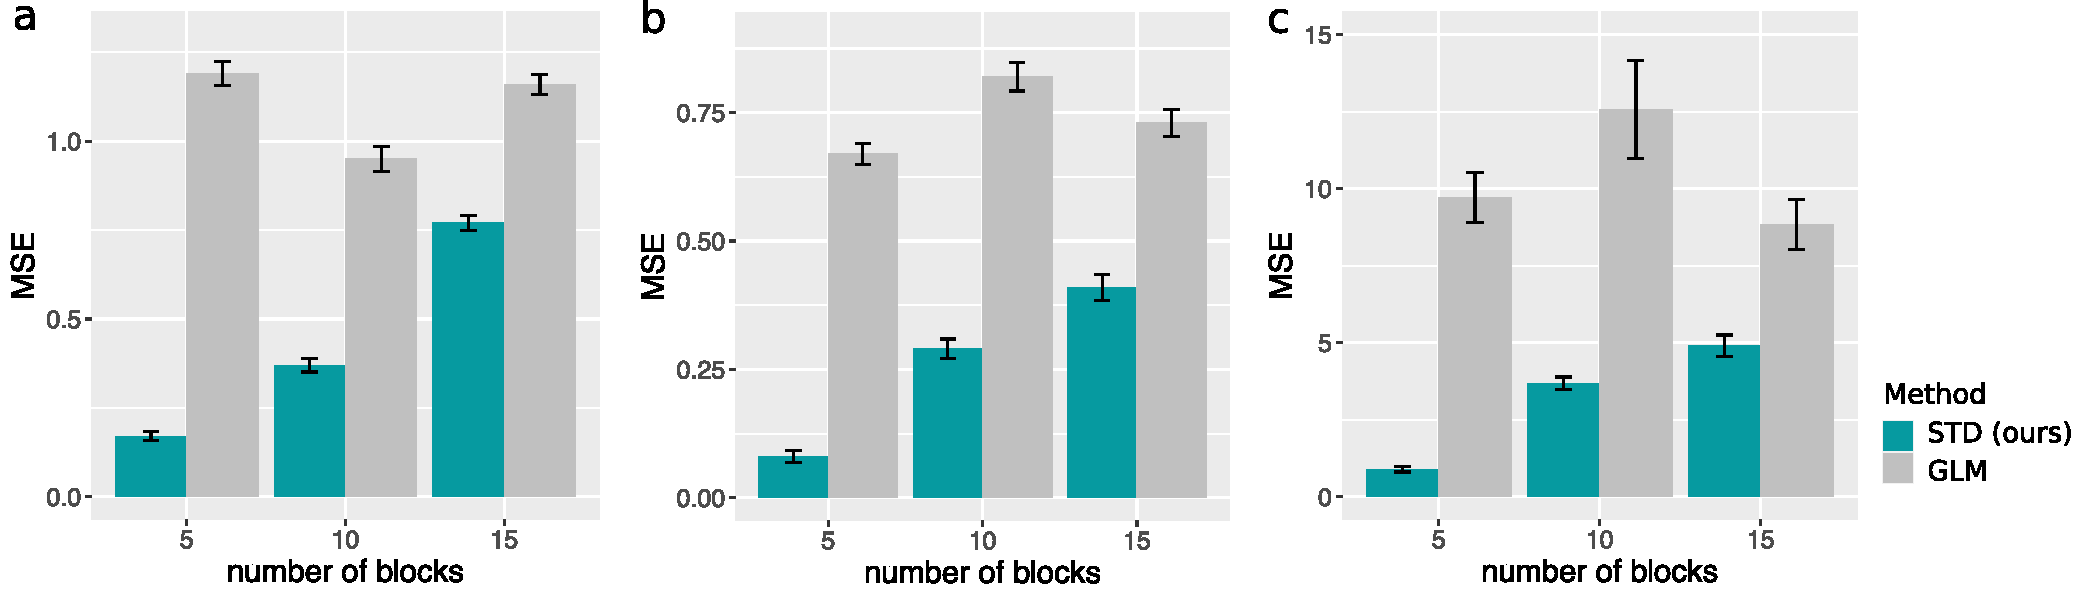
\includegraphics[width=16cm]{compare_GLM.pdf}
\caption{Performance comparison under stochastic block models. The three panels plot the MSE when the response tensors are generated from (a) Gaussian (b) Poisson and (c) Bernoulli models. The $x$-axis represents the number of blocks in the networks. }\label{fig:glm}
\end{figure}


Figure~\ref{fig:glm} compares the MSE of our method with a multiple-response GLM approach. The multiple-response GLM is to regress the dyadic edges, one at a time, on the features, and this model is repeatedly fitted for each edge. As we find in Figure~\ref{fig:glm}, our tensor regression method achieves significant error reduction in all three data types considered. The outperformance is substantial in the presence of large communities; even in the less structured case ($\sim 20/15=1.33$ nodes per block), our method still outer-performs GLM. The possible reason is that the multiple-response GLM approach does not account for the correlation among the edges, and suffers from overfitting. In contrast, the low-rankness in our modeling incorporates the shared information across entries. By selecting the rank in a data-driven way, our method achieves accurate estimation in a wide range of settings. 

\subsection{Comparison with other tensor methods}
We compare our supervised tensor decomposition with three other tensor methods:
\begin{itemize}[noitemsep,topsep=0pt]
\item  Higher-order low-rank regression ({\bf HOLRR},~\citet{rabusseau2016low}) is a least-square based tensor regression that allows features on a single mode. 
\item Higher-order partial least square ({\bf HOPLS},~\citet{zhao2012higher}) is a dimension-reduction method that jointly models a tensor response and a tensor feature. 
\item Subsampled tensor projected gradient ({\bf TPG},~\citet{yu2016learning}) considers the same objective as {\bf HOLRR} but instead uses a different algorithm to solve the problem. 
\end{itemize}
These three methods are the closest algorithms to ours, in that they all relate a data tensor to features using a low-rank structure. The three existing methods allow only Gaussian data, whereas ours is applicable to any exponential family distribution including Gaussian, Bernoulli, Poisson, etc. For fair comparison, we consider Gaussian tensors in the experiment. Because not every method returns the effect estimate $\hat \tB$ as outputs, we measure the accuracy using mean squared prediction error, $\text{MSPE}=(\prod_kd_k)^{-1}\FnormSize{}{\hat \tY-f(\Theta)}^2$, where $f(\Theta)$ is the conditional mean of the tensor, and $\hat \tY$ is the fitted tensor from each method. 

The comparison is assessed from three aspects: (a) benefit of incorporating features from multiple modes; (b) prediction error with respect to sample size; (c) sensitivity of accuracy with respect to model complexity. We use similar simulation setups as in our experiment II, but consider combinations of rank, $\mr=(3,3,3)$ (low) vs.\ $(4,5,6)$ (high), signal $\alpha = 3$ (low) vs.\ $6$ (high), dimension $d$ ranging from 20 to 100 for modes with features, and $d = 20$ for modes without features. Two methods ({\bf STD} and {\bf HOLRR}) require the tensor rank as inputs. For fair comparison, we provide both algorithms the true rank. For algorithms ({\bf HOPLS} and {\bf TPG}) that use different notions of model rank, we use a grid search to set the hyperparameter that gives the best mean square prediction error.

\begin{figure}[ht]
\centering
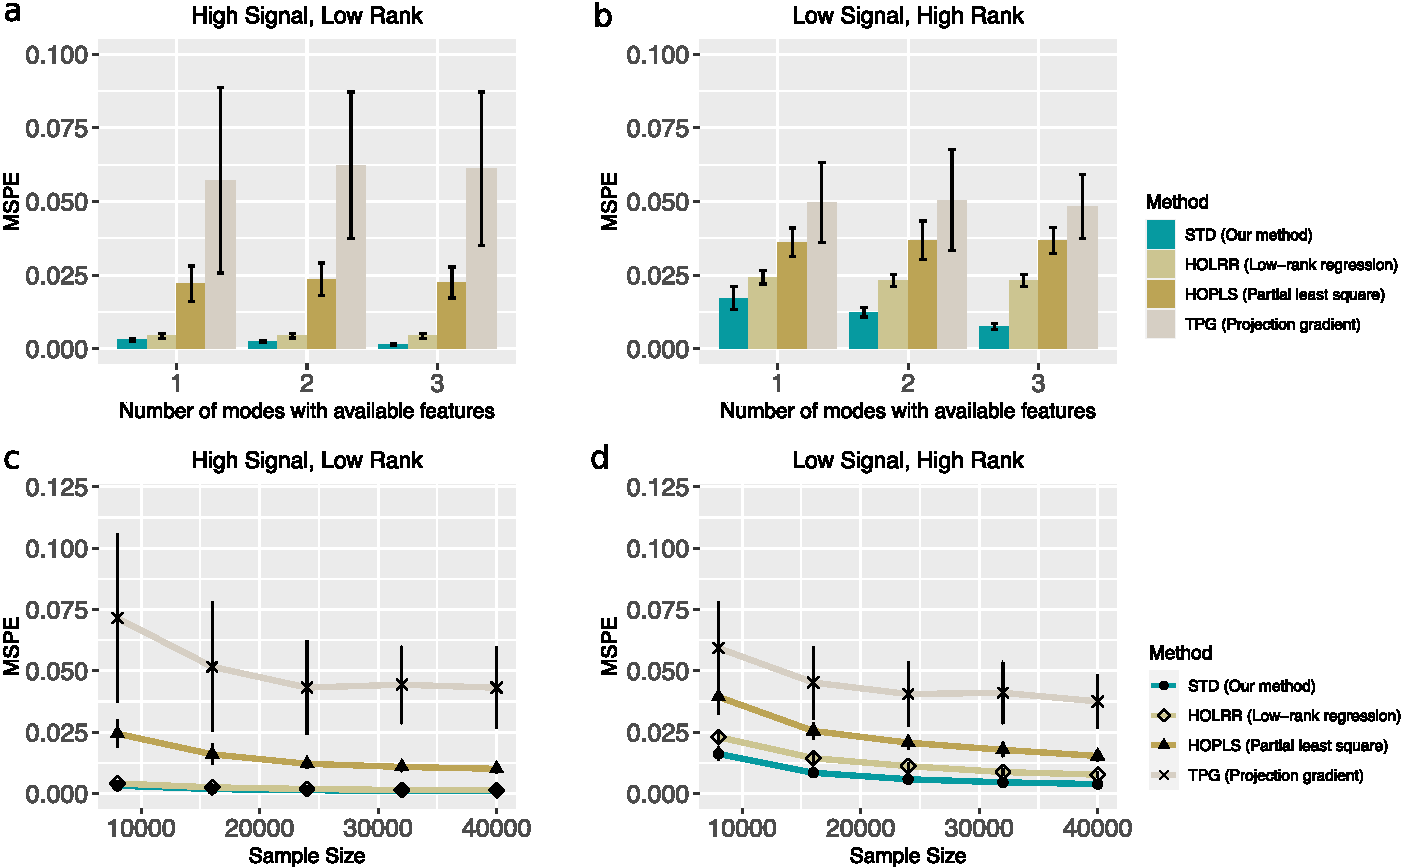
\includegraphics[width=15cm]{compare_alternative.pdf} 
\caption{Comparison between different tensor methods. Panels (a) and (b) plot MSPE versus the number of modes with available features. Panels (c) and (d) plot MSPE versus the effective sample size $d^2$.
We consider rank $\mr=(3,3,3)$ (low), $\mr=(4,5,6)$ (high), and signal $\alpha =3 $ (low), $\alpha=6$ (high).}~\label{fig:compare}
\end{figure}

Figures~\ref{fig:compare}a-b show the averaged prediction error across 30 replicates. We see that our {\bf STD} outperforms others, especially in the low-signal, high-rank setting. As the number of informative modes (i.e., modes with available features) increases, the {\bf STD} exhibits a substantial reduction in error whereas others remain unchanged (Figure~\ref{fig:compare}b). This showcases the benefit of incorporation of multiple features. Note that our method {\bf STD} is most comparable to {\bf HOLRR} when there is only a single informative mode. In such a case, both methods share a same cost function but have different algorithms. {\bf STD} alternates between informative and non-informative modes, whereas {\bf HOLRR} approximates the non-informative modes without alternating. The accuracy gain in Figure~\ref{fig:compare} demonstrates the benefit of alternating algorithm -- incorporation of informative modes also improves the estimation in the non-informative modes. 


Figures~\ref{fig:compare}c-d compare the prediction error with respect to effective sample size when only one mode has side information. In the high-signal low-rank setting, our method has similar performance as {\bf HOLRR}, and the improvement becomes more pronounced in the low-signal high-rank setting. The latter setting is harder because of the higher inter-mode complexity, and our {\bf STD} method shows the advantage in addressing this challenge. 


\section{Data analyses}\label{sec:data}
We apply our supervised tensor decomposition to two datasets. The first application studies the brain networks in response to individual attributes (i.e.,\ feature on one mode), and the second application focuses on multi-relational network analysis with dyadic attributes (i.e.,\ features on two modes). 

\subsection{Application to human brain connection data}
The Human Connectome Project (HCP) aims to build a network map that characterizes the anatomical and functional connectivity within healthy human brains~\citep{HCP}. 
%We analyze the structural connectivity patterns among 68 brain regions for 136 individuals from HCP. 
We follow the preprocessing procedure as in~\cite{zhang2018mapping} and parcellate the brain into 68 regions of interest~\citep{desikan2006automated}. The dataset consists of 136 brain structural networks, one for each individual. Each brain network is represented as a 68-by-68 binary matrix, where the entries encode the presence or absence of fiber connections between the 68 brain regions. We consider four individual features: gender (65 females vs.\ 71 males), age 22-25 ($n=35$), age 26-30 ($n=58$), and age 31+ ($n=43$). The preprocessed dataset is released in our R package \texttt{tensorregress}. The goal is to identify the connection edges that are affected by individual features. A key challenge in brain network is that the edges are correlated; for example, the nodes in edges may be from a same brain region, and it is of importance to take into account the within-dyad dependence. 

\begin{figure}[!h]
\centering

\includegraphics[width=16cm]{HCP.pdf}
\caption{Top edges with large effects. (a) Global effect; (b) Female effect; (c) Age 22-25; (d) Age 31+. Red edges represent positive effects and blue edges represent negative effects. The edge-width is proportional to the magnitude of the effect size.
}\label{fig:brain}
\vspace{1cm}
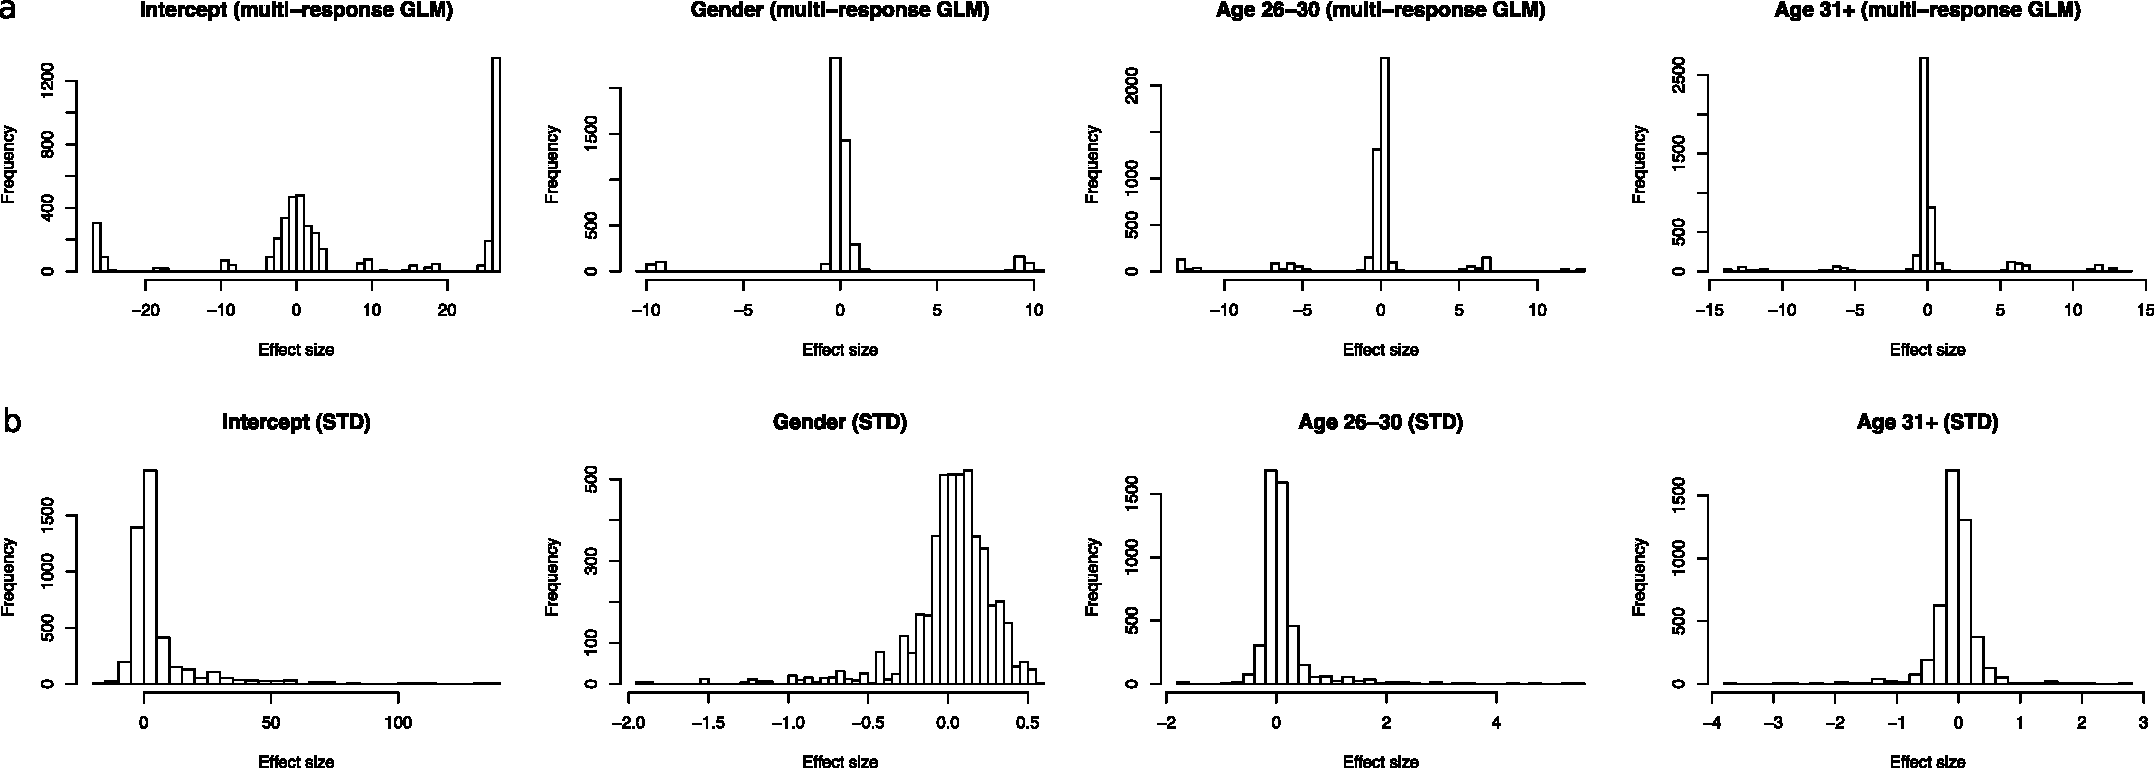
\includegraphics[width=16cm]{compare_HCP.pdf}
\caption{Comparison of estimated feature effects the HCP data using (a) multi-response GLM and (b) supervised tensor decomposition (STD). }\label{fig:s1}
\end{figure}


We perform the supervised tensor decomposition to the HCP data. %The data tensor is binary, $\tY\in\{0,1\}^{68\times 68\times 136}$, and the features are of dimension 4 on the 3$^{\text{rd}}$ mode. 
The BIC selection suggests a rank $\mr=(10,10,4)$ with quasi log-likelihood $\tL_{\tY}=-174654.7$. We utilize the sum-to-zero contrasts in coding the feature effects, and depict only the top 3\% edges whose connections are non-constant across the sample. Figure~\ref{fig:brain} shows the top edges with high effect size, overlaid on the Desikan atlas brain template~\citep{desikan2006automated}. We find that the global connection exhibits clear spatial separation, and that the nodes within each hemisphere are more densely connected with each other (Figure~\ref{fig:brain}a). In particular, the superior-temproal (\emph{SupT}), middle-temporal (\emph{MT}) and Insula are the top three popular nodes in the network. Interestingly, female brains display higher inter-hemispheric connectivity, especially in the frontal, parental and temporal lobes (Figure~\ref{fig:brain}b). This is in agreement with a recent study showing that female brains are optimized for inter-hemispheric communication~\citep{ingalhalikar2014sex}. We find several edges with declined connection in the group Age 31+. Those edges involve Frontal-pole (\emph{Fploe}), superior-frontal (\emph{SupF}) and Cuneus nodes. The Frontal-pole region is known for its importance in memory and cognition, and the detected decline with age further highlights its biological importance. 

%\begin{figure}[h]
%\centering
%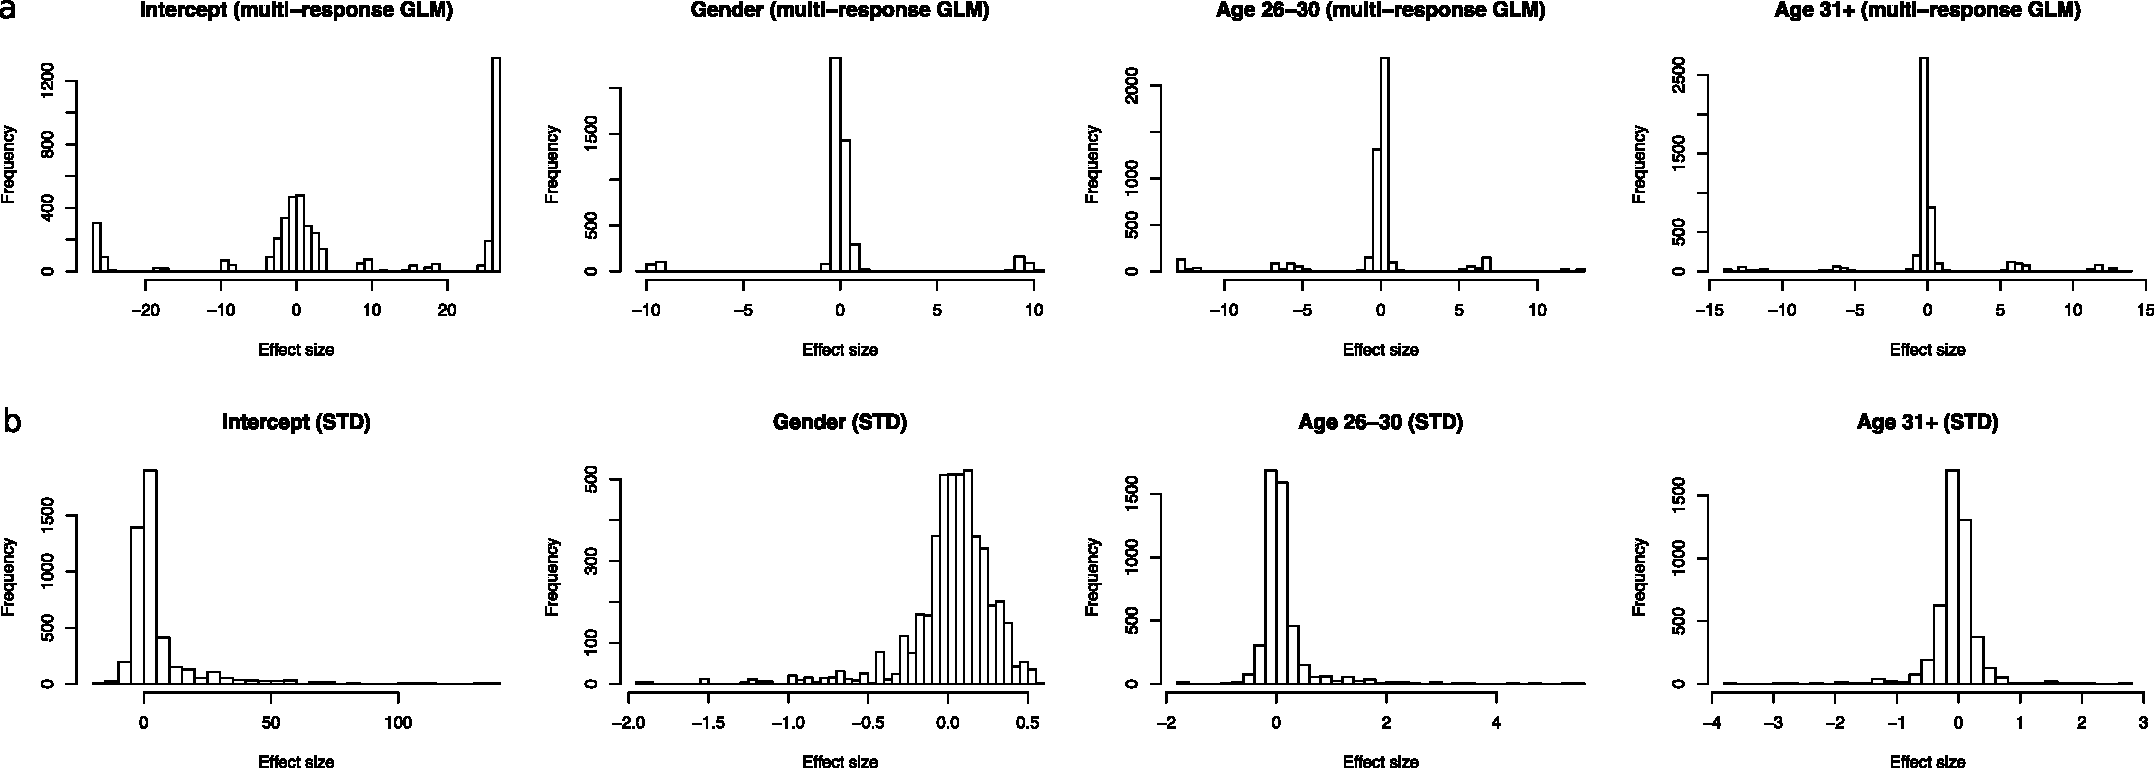
\includegraphics[width=16cm]{compare_HCP.pdf}
%\caption{Comparison of feature effect estimation in the HCP data.}\label{fig:s1}
%\end{figure}


Figure~\ref{fig:s1} compares the estimated coefficients from our method with those from multiple-response GLM approach. The multiple-response GLM is to regress the brain edges, one at a time, on the individual-level features, and this model is repeatedly fitted for every edge $\in [68]\times [68]$. As we can see in the figure, our tensor decomposition method shrinkages the coefficients towards center, thereby implicitly enforcing the sharing between feature effects. 



\subsection{Application to political relation data}

The second application studies the multi-relational networks with node-level attributes. We consider \emph{Nations} dataset~\citep{nickel2011three} which records 56 relations among 14 countries between 1950 and 1965. The multi-relational networks can be organized into a $14 \times 14 \times 56$ binary tensor, with each entry indicating the presence or absence of an action, such as ``sending tourist to'', ``export'', ``import'', between countries. The 56 relations span the fields of politics, economics, military, religion, etc. In addition, country-level attributes are also available, and we focus on the following six features: \emph{constitutional, catholics, law ngo, political leadership, geography}, and \emph{medicine ngo}. The goal is to identify the variation in connections due to country-level attributes and their interactions. One of the key features is that the 56 relations are correlated, and we would like to take it into account in assessing the feature effects. 

We apply our tensor model to the \emph{Nations} data. The multi-relational network $\tY$ is a binary data tensor, and the country attributes $\mX\in\mathbb{R}^{14\times 6}$ are features on both the 1$^\text{st}$ and 2$^\text{nd}$ modes. The BIC criterion suggests a rank $\mr=(4,4,4)$ for the coefficient tensor $\tB\in\mathbb{R}^{6\times 6 \times 56}$. 
We perform the supervised tensor decomposition and obtain the dimension reduction matrices $\hat \mM_k$ from the model. Then we apply $K$-mean clustering to dimension reduction matrix on each of the modes. Table~\ref{fig:s1} shows the K-means clustering of the 56 relations based on the dimension reduction matrix on the 3$^\text{rd}$ mode. We find that the relations reflecting the similar aspects of actions are grouped together. In particular, Cluster I consists of military relations such as \emph{violentactions}, \emph{warnings} and \emph{militaryactions}; Clusters II and III capture the economic relations such as \emph{economicaid, booktranslations, tourism}; and Cluster IV represents the political alliance and territory relations. 

\begin{figure}[!h]
\centering
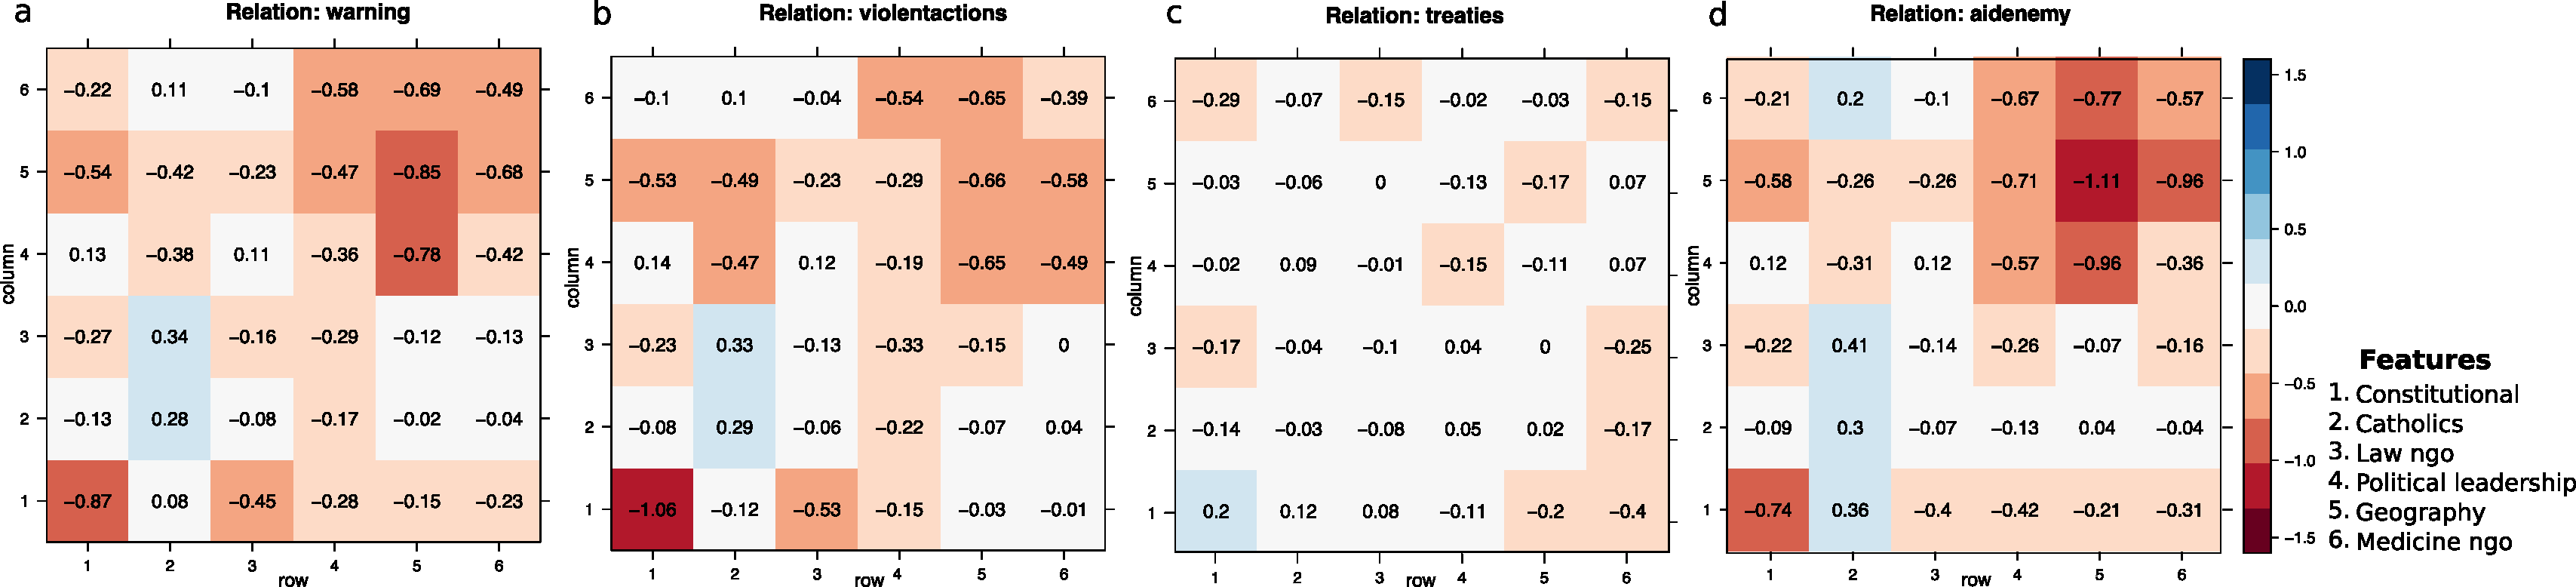
\includegraphics[width=16cm]{coef.pdf}
\caption{Estimated feature effects in the \emph{Nations} data analysis. Panels (a)-(d) represent the estimated effects of country-level attributes towards the connection probability, for relations \emph{warning}, \emph{violentactions}, \emph{treaties}, and \emph{aidenemy}, respectively. }\label{fig:est}
\end{figure}


\begin{table}[!h]
\resizebox{\textwidth}{!}{%
\begin{tabular}{c|c|l}
 & Category & \multicolumn{1}{c}{Relations}\\
\hline
\multirow{2}{*}{ I}  & \multirow{2}{*}{Military} & warning, violentactions, militaryactions, duration, negativebehavior, protests, severdiplomatic \\
&&timesincewar, commonbloc0, commonbloc1, blockpositionindex,  expeldiplomats\\   
\hline
\multirow{2}{*}{II}& \multirow{2}{*}{Emigrant} & emigrants, emigrants3, relemigrants, accusation, nonviolentbehavior, ngoorgs, commonbloc2, intergovorgs3\\      
&&releconomicaid, relintergovorgs, relngo,  students, relstudents, economicaid, negativecomm, militaryalliance \\
\hline
\multirow{3}{*}{ III} & \multirow{3}{*}{Economics} & treaties, reltreaties, officialvisits, exportbooks, relexportbooks, booktranslations, relbooktranslations\\
&&boycottembargo, weightedunvote, unweightedunvote, reltourism, tourism, tourism3, exports, exports3  \\
&&relexports, intergovorgs, ngo, embassy, reldiplomacy, timesinceally, independence, conferences, dependent\\
\hline
IV & Territory &aidenemy, lostterritory, unoffialacts, attackembassy\\
\hline
\end{tabular}
}
\caption{$K$-means clustering of relations based on dimension reduction on the 3$^\text{rd}$ mode. }\label{tab:s1}
\end{table}


To investigate the effects of dyadic attributes towards connections, we depict the estimated coefficients $\hat \tB=\entry{\hat b_{ijk}}$ for several relation types (Figure~\ref{fig:est}). Note that the each entry $\hat b_{ijk}$ estimates the contribution, at the logit scale, of feature pair $(i,j)$ ($i$th feature for the ``sender'' country and $j$th feature for the ``receiver'' country) towards the connection of relation $k$. Several interesting findings emerge from the observation. We find that relations belonging to a same cluster tend to have similar feature effects. For example, the relations ``warning'' and ''violentactions'' are classified into Cluster I, and both exhibit similar effect patterns (Figures~\ref{fig:est}a-b). Moreover, the feature \emph{constitutional} has a strong effect in the relation ``violentactions'' and ``warning'', whereas the effect is weaker in the relation ``treaties''. The result is plausible because the constitutional attributes affect political actions more often than economical actions. The entries in $\tB$ are useful for revealing interaction effects in a context-specific way. 
%For a given relation $k$, the off-diagonal entries in the matrix $\hat \tB(\colon,\colon,k)$ represent the pairwise interactions between features. 
From Figure~\ref{fig:est}, we find a strong interaction between \emph{geography} and \emph{political leadership} in the relation ``warning'', and a strong interaction between \emph{geogrphy} and \emph{medicine ngo} in the relation ``aidenemy''. The relation-specific effect pattern showcases the applicability of our method in revealing complex interactions. 


\section{Discussion and future work}\label{sec:con}
We have developed a supervised tensor decomposition method with side information on multiple modes. One important challenge of tensor data analysis is the complex interdependence among tensor entries and between multiple features. Our approach incorporates side information as feature matrices in the conditional mean tensor. The empirical results demonstrate the improved interpretability and accuracy over previous approaches. Applications to the brain connection and political relationship datasets yield conclusions with sensible interpretations, suggesting the practical utility of the proposed approach.
 
There are several possible extensions from the work. We have provided accuracy guarantees for parameter estimation in the supervised tensor model. Statistical inference based on tensor decomposition is an important future direction. Measures of uncertainty, such as confidence envelope for space estimation, would be useful. One possible approach would be performing parametric bootstrap~\citep{tibshirani1993introduction} to assess the uncertainty in the estimation. 
For example, one can simulate tensors from the fitted low-rank model based on the estimates, and then assess the empirical distribution of the estimates. 
While being simple, bootstrap approach is often computationally expensive for large-scale data. Another possibility is to leverage recent development in debiased inference with distributional characterization~\citep{chen2019inference,xia2019confidence}. This approach has led to fruitful results for matrix data analysis. Uncertainly quantification involving tensors are generally harder than matrices, and establishing distribution theory for tensor estimation remains an open problem.

One assumption made by our method is that tensor entries are conditionally independent given the linear predictor $\Theta$. This assumption can be extended by introducing a more general mixed-effect tensor model. For example, in the special case of Gaussian model, we can model the first two moments of data tensor using
\begin{align}\label{eq:extention}
\mathbb{E}(\tY|\mX_1,\ldots,\mX_K)&=\tC\times\mM_1\times \cdots \times \mM_K,\\
 \text{Var}(\tY|\mX_1,\ldots,\mX_K)&=\mPhi_1\otimes \cdots \otimes \mPhi_K,
\end{align}
where $\mPhi_k\in\mathbb{R}^{d_k\times d_k}$ is the unknown covariance matrix on the mode $k\in[K]$. For general exponential family, an additional mean-variance relationship should also be considered. The joint estimation of mean model $\Theta$ and variance model $\mPhi_k$ will lead to more efficient estimation in the presence of unmeasured confounding effects. However, the introduction of unknown covariance matrices $\mPhi_k$ dramatically increases the number of parameters in the problem. Suitable regularization such as graphical lasso or specially-structured covariance assumptions should be considered. The extension of tensor modeling with heterogeneous mixed-effects will be an important future direction. 

Although we have presented the supervised tensor decomposition in the context of order-3 data tensors, the framework applies to more general multi-way datasets. One possible extension is the integrative analysis of omics data, in which multiple types of omics measurements (gene expression, DNA methylation, microRNA) are collected in the same set of individuals~\citep{lock2013joint,wang2019three}. In such a case, the observation is a stack of data matrices, which may not be of the same dimension. 
%One possible extension is to impose linked dimension reduction among different data matrices, and incorporate side information as features in the joint decomposition. 
Other applications include time-series tensor data with multiple side information. Exploiting the benefits and properties of the supervised tensor decomposition in specialized task will boost scientific discoveries.


\bigskip
\begin{center}
{\large \bf SUPPLEMENTARY MATERIALS}
\end{center}

\begin{description}
\item[Supplementary notes:]  technical proofs and additional simulation results.
\item[Data and software:] %R-package \texttt{tensorregress} performs our supervised tensor decomposition method. 
Our simulation code, R-package \texttt{tensorregress}, and datasets used in the paper are available at \url{https://CRAN.R-project.org/package=tensorregress} 
We also provide R scripts for reproducing all numbers in Figures 2-8 and Tables 2-3 in the paper.
\end{description}

\bibliography{tensor_wang}
\bibliographystyle{apalike}


\end{document}
